%!TEX root=../../main.tex

\chapter{Inference for categorical data}
\label{inferenceForCategoricalData}

Previous chapters discussed methods of inference for numerical data; in this chapter, those methods are extended to categorical data, such as binomial proportions or data in two-way tables. While various details of the methods may change, such as the calculations for a test statistic or the distributions used to find a $p$-value, the core ideas and principles behind inference remain the same.  

Categorical data arise frequently in medical research because disease outcomes and patient characteristics are often recorded in natural categories such as types of treatment received, whether or not disease advanced to a later stage, or whether or not a patient responded initially to a treatment. In the simplest settings, a binary outcome (yes/no, success/failure, etc)  is recorded for a single group of participants, in hopes of learning more about the population from which the participants were drawn.  The binomial distribution is often used for the statistical model in this setting, and inference about the binomial probability of success provides information about a population proportion $p$.   In more complex settings, participant characteristics are recorded in a factor variable with two or more levels, and the outcome or response variable itself has two or more levels.  In these instances, data are usually summarized in two-way tables with two or more rows and two or more columns.

As with all methods of inference, it is important to understand how the data were collected and whether the data is a random sample from a well-identified population, at least approximately.  This issue is at least as important as the formulas for test statistics and confidence intervals, and is often overlooked.

The next section illustrates the use of inference with binomial data in a current line of research in cancer therapy.  Be careful about the notation in this chapter - since $p$ is the standard notation for a population proportion or probability, $p$ does double duty in this chapter as a population parameter and significance level.  The notation is unfortunate but commonly used.

%__________________
\section{Inference for a single proportion}
\label{singleProportion}

Advanced melanoma is an aggressive form of skin cancer that until recently was uniformly fatal.  Historically, some cancers, including melanoma, have stopped progressing or disappeared altogether  when a patient's immune system successfully mounted a response to the cancer. During the last several decades, those observations led to research into therapies that might trigger an immune response in cancer.  Some of the most notable successes have been in melanoma, particularly with two therapies nivolumab and ipilimumab\footnote{The mab suffix in these therapies stands for monoclonal antibody, a therapeutic agent made by identical immune cells that are all clones of a unique parent cell from a patient}.

A 2013 report in the New England Journal of Medicine\footnote{N Engl J Med 2013;369:122-33. DOI: 10.1056/NEJMoa1302369} by Wolchok et al. reported the results of a study in which patients were treated with both of the new regimens.  Fifty-three patients were given the new regimens concurrently, and the response to therapy could be evaluated in 52 of the 53.  Of the 52 evaluable patients, 21 (40\%) experience a response according to commonly accepted criteria.  In previous studies, the proportion of patients responding to one of these agents was 30\% or less.  How might one compare these data with past experience?

The data are from this study are binomial data, with success defined as a good response to therapy. Suppose the number of patients who respond in a study like this is represented by the random variable $X$, where $X$ is binomial with parameters $n$ (the number of trials, where each trial is represented by a patient) and $p$, the unknown population parameter of response. From formulas discussed in Chapter~\ref{modeling}, the mean of $X$ is $np$ and the standard deviation of $X$ is $\sqrt{np(1-p)}$.

Inference about $p$ is based on the sample proportion $\hat{p}$, where $\hat{p} = X/n$. In this case, $\hat{p} = 21/52 = 0.404$. If the sample proportion is nearly normal distributed, the normal approximation to the binomial distribution can be used to conduct inference; this method is commonly used since normal probability tables are easily available in either paper or electronic form.  When $X$ does not have an approximately normal distribution, exact inference can  based on the binomial distribution for $X$.  Both the normal approximation and exact methods are covered in this chapter.



\subsection{Inference using the normal approximation}

A sample proportion can be described as a sample mean. If each success  is represented as a \texttt{1} and each failure as a \texttt{0}, then the sample proportion is the mean of these 52 numerical outcomes:
\begin{eqnarray*}
\hat{p} = \frac{\ 0 + 1 + 1 + \cdots + 0\ }{52} = 0.404.
\end{eqnarray*}
The distribution of $\hat{p}$ is nearly normal when the distribution of successes and failures is not too strongly skewed for the sample size.

\begin{termBox}{\tBoxTitle{Conditions for the sampling distribution of $\hat{p}$ being nearly normal}
The sampling distribution for $\hat{p}$, calculated from a sample of size $n$ from a population with a success proportion $p$, is nearly normal when
\begin{enumerate}
\item the sample observations are independent and
\item at least 10 successes and 10 failures are expected in the sample, i.e. $np\geq10$ and $n(1-p)\geq10$. This is called the \term{success-failure condition}.
\end{enumerate}

If these conditions are met, then the sampling distribution of $\hat{p}$ is approximately normal with mean $p$ and standard error
\index{standard error (SE)!single proportion}
\begin{eqnarray}
SE_{\hat{p}} = \sqrt{\frac{p(1-p)}{n}}
\label{seOfPHat}
\end{eqnarray}}
\end{termBox}\marginpar[\raggedright\vspace{-53mm}

$\hat{p}$\vspace{0mm}\\\footnotesize sample\\proportion\vspace{3mm}\\\normalsize$p$\vspace{0mm}\\\footnotesize population\\proportion]{\raggedright\vspace{-53mm}

$\hat{p}$\vspace{0mm}\\\footnotesize sample\\proportion\vspace{3mm}\\\normalsize$p$\vspace{0mm}\\\footnotesize population\\proportion}

When conducting inference, the population proportion $p$ is unknown, and the sample proportion $\hat{p}$ can be substituted for $p$ to check the success-failure condition and compute the standard error.

\subsubsection{Confidence intervals for a proportion}
\label{confIntForPropSection}

\index{point estimate!single proportion}

When using the normal approximation to the sampling distribution of $\hat{p}$, a confidence interval for a proportion has the same structure as a confidence interval for a mean; it is centered at the point estimate, with a margin of error calculated from the standard error and appropriate $z^{\star}$ value.  The formula for a 95\% confidence interval is
\[
     \hat{p} \pm 1.96 \sqrt{\frac{p(1-p)}{n}}.
\]


\begin{example}{Using the normal approximation, construct an approximate 95\% confidence interval for the response probability for patients with advanced melanoma who were administered the combination of nivolumab and ipilimumab.}

The independence and success-failure assumptions should be checked first.  Since the outcome of one patient is unlikely to influence that of other patients, the observations are independent.  The success-failure condition is satisfied since $n\hat{p} = (52)(.404) = 21  > 10$ and $n\hat{p}(1 - \hat{p}) = (52)(.596) = 31  > 10$.

The point estimate for the response probability, based on a sample of size $n = 52$, is $\hat{p} = 0.404$. For a 95\% confidence interval, $z^{\star} = 1.96$. The margin of error is estimated as: $\sqrt{\frac{\ \hat{p}(1-\hat{p})\ }{n}} = \sqrt{\frac{(0.404)(1-0.404)}{52}} = 0.068$.  The confidence interval is

\[0.404 \pm 1.96 (0.068) \rightarrow (0.27, 0.54) \]

The approximate 95\% confidence interval for $p$, the population response probability to CAR-T cells among patients with relapsed or refractory lymphoma is  (0.27, 0.54), or (27\%, 54\%).  

\end{example}

Patients with a form of cancer who participate in clinical trials at research samples are unlikely to be a random sample of patients from the disease, since the patients or their physicians must be aware of the trial, and patients must be well enough to travel to a major medical center and be willing to receive an experimental therapy that may have serious side effects.  Investigators are aware that the hypothetical response probability of the population of patients with advanced melanoma treated with new therapies on a clinical trial may be different than the observed proportion of patients responding in a clinical trial.  Study teams try to minimize these differences by using a research protocol with a detailed specification of the characteristics of the disease used to decide if a patient was eligible for the study and assuming that other potential differences do not have a large effect on outcome.  But there can be no guarantee that systematic differences between a study sample and an overall population do not influence the results.  Small, initial studies in which there is no control group like the one described here early steps in exploring the value of a new therapy and are used to justify further study of a treatment when the results are substantially different than expected.  The largest observed response rate in previous trials of 30\% is not outside the confidence interval from this study and but the results of the study were considered adequate justification for continued research on this treatment.




\begin{exercise}
In New York City on October 23rd, 2014, a doctor who had recently been treating Ebola patients in Guinea went to the hospital with a slight fever and was subsequently diagnosed with Ebola. Soon after, a survey conducted by the Marist Poll, an organization with a carefully designed methodology for drawing random samples from identified populations, found that 82\% of New Yorkers favored a "mandatory 21-day quarantine for anyone who has come in contact with an Ebola patient."\footnote{\oiRedirect{textbook-maristpoll_ebola_201410}{Poll ID NY141026 on maristpoll.marist.edu}.} a) Verify that the sampling distribution of $\hat{p}$ is nearly normal. b) Construct a 95\% confidence interval for $p$, the proportion of New York adults who supported a quarantine for anyone who has come into contact with an Ebola patient.\footnote{a) The poll is based on a simple random sample and consists of fewer than 10\% of the adult population of New York, which makes independence a reasonable assumption. The success-failure condition is satisfied since, $1042(0.82) > 5$ and $1042(1-0.82) > 5$. b) $0.82 \pm 1.96\sqrt{\frac{0.82(1-0.82)}{1042}} \rightarrow (0.796, 0.844)$. }
\end{exercise}


\subsubsection{Hypothesis testing for a proportion}
\label{htForPropSection}


Just as with inference for population means, confidence intervals for population proportions can be used when deciding whether to reject a null hypothesis. It is useful in most settings, however, to also calculate the $p$-value for a test as a measure of the strength of the evidence contradicting the null hypothesis.

When using the normal approximation for the distribution of $\hat{p}$ to conduct a hypothesis test, one should always verify that $\hat{p}$ is nearly normal under $H_0$ by checking the independence and success-failure conditions. Since a hypothesis test is based on the distribution of the test statistic under the null hypothesis, the success-failure condition is checked using the null proportion $p_0$, not the estimate $\hat{p}$. 

According to the normal approximation to the binomial distribution, the number of successes in $n$ trials is normally distributed with mean $np_0$ and standard deviation $\sqrt{np(1-p_0)}$. This approximation is valid when $np_0$ and $n(1-p_0)$ are both at least 10.\footnote{The normal approximation to the binomial distribution was discussed in Section~\ref{binomialModel} of Chapter~\ref{modeling}.} 

Under the null hypothesis, the sample proportion $\hat{p} = X/n$ has distribution 
\[N \left(p_0, \sqrt{\frac{p_0(1-p_0)}{n}} \right).\]

The test statistic $z$ for null the hypothesis $H_0: p = p_0$ is based on a sample of size $n$ is 
\begin{align*}
  z &= \dfrac{\text{point estimate - null value}}{SE} \\
    &= \dfrac{\hat{p} - p_0}{\sqrt{\frac{(p_0)(1-p_0)}{n}}}. 
\end{align*}

\begin{example}{Suppose that out of a cohort of 120 patients with stage 1 lung cancer at the Dana-Farber Cancer Institute (DFCI), 80 of the patients survive at least 5 years, and suppose that National Cancer Institute statistics indicate that the 5-year survival probability for stage 1 lung cancer patients nationally is 0.60. Do the data collected from 120 patients support the claim that the DFCI population with this disease has a different 5-year survival probability than the national population?}

Test the hypothesis $H_0: p = 0.60$ versus the alternative, $H_A: = p \neq 0.60$, using $\alpha = 0.05$. If we assume that the outcome of one patient at DFCI does not influence the outcome of other patients, the independence condition is met, and the success-failure condition is satisfied since $(120)(0.60) = 80 > 5$ and $(120)(1-0.67) = 40 > 5$ The test statistic is the $z$-score of the point estimate: 

\[z = \dfrac{\text{point estimate - null value}}{SE} = \dfrac{0.67 - 0.60}{\sqrt{\frac{(0.60)(1-0.60)}{120}}} = 1.57 \]

The $p$-value is 0.12; since the $p$-value is greater than 0.05, there is insufficient evidence to reject $H_0$ in favor of $H_A$. There is not convincing evidence that the survival probability at DFCI differs from the national rate.

\end{example}

\begin{example} {Using the data from the study in advanced melanoma, use the normal approximation to the sampling distribution of $\hat{p}$ to test the null hypothesis that the response probability to the novel combined therapy is 30\% against a two sided alternative.}

The test statistic has value 
\[
z = (0.404 - 0.30)/\sqrt{(0.30)(0.70)/52} = 1.64. 
\] 

The two-sided p-value is $P(|Z| \geq 1.64) = 0.10$. The null hypothesis is not rejected.  This is consistent with the fact that 0.30 was not outside the 95\% confidence interval for the response probability.

\end{example}

\begin{exercise} One of the questions on the National Health and Nutrition Examination Survey (introduced in Chapter~\ref{inferenceForNumericalData}) asked participants whether they participated in moderate or vigorous intensity sports, fitness, or recreational activities. In a random sample of 135 adults, 76 answered "Yes" to the question. Based on this evidence, are a majority of American adults physically active?\footnote{The observations are independent. Check success-failure: $np_0 = n(1-p_0) = 135(0.5) > 10$. $H_0: p = 0.5$; $H_A: p > 0.5$. Calculate the $z$-score: $z = \frac{0.56 - 0.50}{\sqrt{\frac{0.5(1-0.5)}{135}}} = 1.39$. The $p$-value is 0.08. Since the $p$-value is larger than 0.05, there is insufficient evidence to reject $H_0$; there is not convincing evidence that a majority of Americans are physically active.}
\end{exercise}


\subsection{Inference using exact methods}

When the normal approximation to the distribution of $\hat{p}$ may not be accurate, inference is based on exact binomial probabilities. With access to a computing package, calculating confidence intervals and $p$-values based on the binomial distribution is relatively easy. Although the logic behind computing a $p$-value is discussed here, the formulas for a confidence interval are complicated and not shown.

The $p$-value for a hypothesis test corresponds to the sum of the probabilities of all events that are or more extreme than the sample result obtained. Let $X$ be a binomial random variable with parameters $n$ and $p_0$, where $\hat{p} = x/n$ and $x$ is the observed number of events. If $\hat{p} \leq p_0$, then the one-tail probability equals $P(X \leq x)$; if $\hat{p} > p_0$, then the one-tail probability equals $P(X \geq x)$. These probabilities are calculated using the approaches from Chapter~\ref{modeling}.

\begin{example}{In 2009, the FDA Oncology Drug Advisory Committee (ODAC) recommended that the drug Avastin be approved for use in glioblastoma, a form of brain cancer. Tumor shrinkage after taking a drug is called a response; out of 85 patients, 24 exhibited a response. Historically, response probabilities for brain cancer drugs were approximately 0.05. Assess whether there is evidence that the response probability for Avastin is different from previous drugs. 		
}	

$H_0: p = 0.05$; $H_A: p \neq 0.05$. Let $\alpha = 0.05$. This is one of those situations where $p$ is doing double duty and (be careful!) the null hypothesis value for the parameter and the significance level $\alpha$ have the same numerical value. 

The independence condition is satisfied, but the success-failure condition is not, since $np_0 = (85)(0.05) = 4.25 < 10$, so this is a setting where exact binomial probabilities should be used to calculate a $p$-value.

The sample proportion $\hat{p}$ equals $x/n = 24/85 = 0.28$. Since $\hat{p} > p_0$, calculate the two-sided $p$-value from $2 \times P(X \geq 24)$, where $X \sim \text{Binom}(85, 0.05)$.

Calculating the $p$-value by hand would be time-consuming and error prone; it is best done in software using, for instance, the R command $pbinom$:

\texttt{2*(1 - pbinom(q = 23, size = 85, p = 0.05))},

which returns value $(5.3486)10^{-12}$.  The FDA staff felt that this highly significant evidence suggesting that the response probability for Avastin is higher than for previous brain cancer drugs was sufficient to justify approval for the use of the drug in that disease.  The decision was a rare one, since the FDA normally requires evidence from two independently conducted randomized trial. 
	
\end{example}



\begin{exercise} Medical consultants assist patients with all aspects of an organ donation surgery, with the goal of reducing the possibility of complications during the medical procedure and recovery. To attract customers, one consultant noted that while the average complication rate for liver donation surgeries in the United States is about 10\%, she has only had 3 out of 62 clients experience complications with liver donor surgeries. Is there evidence to suggest that the rate of complications for her patients is lower than the national average?\footnote{Assume that the 62 patients she is referring to may be viewed as a random sample from her patient population. The sample proportion $\hat{p} = 3/62 = 0.048$. Under the null hypothesis, the expected number of complications is $62(0.10) = 6.2$, so the normal approximation may not be accurate and it is best to use exact binomial probabilities. Since $\hat{p} \leq p_0$, find the $p$-value by calculating $P(X \leq 3)$ when $X$ has a binomial distribution with parameters $n = 62,\, p = 0.10$: $P(X \leq 3) = 0.121$. There is not sufficient evidence to suggest that the rate of complications for her patients is lower than the national average.}
\end{exercise}



\begin{comment}

\textit{JV: This guided practice is from the OI section on small sample hypothesis testing, where they show how to generate the null distribution and $p$-value by simulation, as well as using the binomial method. Could be informative to show the simulation method in the companion, although I do not think it needs to be discussed in this text.}

\end{comment}

%JV: Hid section about choosing sample sizes because it seemed to disrupt the flow of the chapter.

\begin{comment}

\subsection{Choosing a sample size when estimating a proportion}

\index{margin of error|(}

When collecting data, we choose a sample size suitable for the purpose of the study. Often times this means choosing a sample size large enough that the \term{margin of error} -- which is the part we add and subtract from the point estimate in a confidence interval -- is sufficiently small that the sample is useful. More explicitly, our task is to find a sample size $n$ so that the sample proportion is within some margin of error $m$ of the actual proportion with a certain level of confidence.

% For example, the margin of error for a point estimate using 95\% confidence can be written as $1.96\times SE$. We set up a general equation to represent the problem:
%\begin{align*}
%ME = z^{\star}SE \leq m
%\end{align*}
%where $ME$ represented the actual margin of error and $z^{\star}$ was chosen to correspond to the confidence level. The standard error formula is specified to correspond to the particular setting. For instance, in the case of means, the standard error was given as $\sigma / \sqrt{n}$. In the case of a single proportion, we use $\sqrt{p(1-p) / n\ }$ for the standard error.

\begin{example}{A university newspaper is conducting a survey to determine what fraction of students support a \$200 per year increase in fees to pay for a new football stadium. How big of a sample is required to ensure the margin of error is smaller than 0.04 using a 95\% confidence level?}
The margin of error for a sample proportion is
\begin{align*}
z^{\star} \sqrt{\frac{p (1 - p)}{n}}
\end{align*}
Our goal is to find the smallest sample size $n$ so that this margin of error is smaller than $m=0.04$. For a 95\% confidence level, the value $z^{\star}$ corresponds to 1.96:
\begin{align*}
1.96\times \sqrt{\frac{p(1-p)}{n}} \ < \ 0.04
\end{align*}
There are two unknowns in the equation: $p$ and $n$. If we have an estimate of $p$, perhaps from a similar survey, we could enter in that value and solve for $n$. If we have no such estimate, we must use some other value for $p$. It turns out that the margin of error is largest when $p$ is 0.5, so we typically use this \emph{worst case value} if no estimate of the proportion is available:
\begin{align*}
	1.96\times \sqrt{\frac{0.5(1-0.5)}{n}} &\ < \ 0.04 \\
	1.96^2\times \frac{0.5(1-0.5)}{n} &\ < \ 0.04^2 \\
	1.96^2\times \frac{0.5(1-0.5)}{0.04^2} &\ < \ n \\
	600.25 &\ < \  n
\end{align*}
We would need over 600.25 participants, which means we need 601 participants or more, to ensure the sample proportion is within 0.04 of the true proportion with 95\% confidence.
\end{example}

When an estimate of the proportion is available, we use it in place of the worst case proportion value,~0.5.

\begin{example}{A manager is about to oversee the mass production of a new tire model in her factory, and she would like to estimate what proportion of these tires will be rejected through quality control. The quality control team has monitored the last three tire models produced by the factory, failing 1.7\% of tires in the first model, 6.2\% of the second model, and 1.3\% of the third model. The manager would like to examine enough tires to estimate the failure rate of the new tire model to within about 2\% with a 90\% confidence level.
\begin{enumerate}
\setlength{\itemsep}{0mm}
\item[(a)] There are three different failure rates to choose from. Perform the sample size computation for each separately, and identify three sample sizes to consider.
\item[(b)] The sample sizes vary widely. Which of the three would you suggest using? What would influence your choice?
\end{enumerate}}
(a)~For a 90\% confidence interval, $z^{\star} = 1.65$, and since an estimate of the proportion 0.017 is available, we'll use it in the margin of error formula: %use theFor the 1.7\% estimate of $p$, we estimate the appropriate sample size as follows:
\begin{align*}
1.65\times \sqrt{\frac{0.017(1-0.017)}{n}} &\ < \ 0.02 \\
113.7 &\ < \ n
\end{align*}
For sample size calculations, we always round up, so the first tire model suggests 114 tires would be sufficient.

A similar computation can be accomplished using 0.062 and 0.013 for $p$, and you should verify that using these proportions results in minimum sample sizes of 396 and~88 tires, respectively.

(b) We could examine which of the old models is most like the new model, then choose the corresponding sample size. Or if two of the previous estimates are based on small samples while the other is based on a larger sample, we should consider the value corresponding to the larger sample. There are also other reasonable approaches.
\end{example}

\index{data!Congress approval rating|(}

\begin{exercise}
A recent estimate of Congress' approval rating was 19\%.\footnote{\oiRedirect{textbook-congress_at_19_in_May2015}{www.gallup.com/poll/183128/five-months-gop-congress-approval-remains-low.aspx}} What sample size does this estimate suggest we should use for a margin of error of 0.04 with 95\% confidence?\footnote{We complete the same computations as before, except now we use $0.19$ instead of $0.5$ for $p$:
\begin{align*}
1.96\times \sqrt{\frac{p(1-p)}{n}} \approx
1.96\times \sqrt{\frac{0.19(1-0.19)}{n}} &\leq 0.04 \qquad\to\qquad n \geq 369.5
\end{align*}
A sample size of 370 or more would be reasonable. (Reminder: always round up for sample size calculations!)}

\index{data!Congress approval rating|)}
\index{margin of error|)}

\end{exercise}

\end{comment}

%__________________
\section{Inference for the difference of two proportions}
\label{differenceOfTwoProportions}

Just as inference can be done with the difference of two means, conclusions can also be drawn about the difference of two population proportions: $p_1 - p_2$. 

\subsection{Sampling distribution of the difference of two proportions}

The normal model can only be applied to $\hat{p}_1 - \hat{p}_2$ if the sampling distribution for each sample proportion is nearly normal, and if the samples are independent. 

\begin{termBox}{\tBoxTitle{Conditions for the sampling distribution of $\hat{p}_1 - \hat{p}_2$ to be normal}
The difference $\hat{p}_1 - \hat{p}_2$ tends to follow a normal model when
\begin{itemize}
\setlength{\itemsep}{0mm}
\item the two samples are independent of each other, and
\item each proportion separately follows a normal model. This condition is satisfied when $np_1 \geq 10$ and $np_2 \geq 10$.
\end{itemize}
The standard error of the difference in sample proportions is
\index{standard error (SE)!difference in proportions}
\begin{eqnarray}
SE_{\hat{p}_1 - \hat{p}_2}
	= \sqrt{SE_{\hat{p}_1}^2 + SE_{\hat{p}_2}^2}
	= \sqrt{\frac{p_1(1-p_1)}{n_1} + \frac{p_2(1-p_2)}{n_2}}
\label{seForDiffOfProp}
\end{eqnarray}
where $p_1$ and $p_2$ represent the population proportions, and $n_1$ and $n_2$ represent the sample sizes.}
\end{termBox}


\subsection{Confidence intervals for $p_1 -p_2$}

When calculating confidence intervals for a difference of two proportions using the normal approximation to the binomial, the two sample proportions are used to verify the success-failure condition and to compute the standard error.

\begin{example}{The way a question is phrased can influence a person's response. For example, Pew Research Center conducted a survey with the following question:\footnote{\oiRedirect{textbook-health_care_bill_2012}{www.people-press.org/2012/03/26/public-remains-split-on-health-care-bill-opposed-to-mandate}. Sample sizes for each polling group are approximate.}
\begin{quote}
As you may know, by 2014 nearly all Americans will be required to have health insurance. [People who do not buy insurance will pay a penalty] while [People who cannot afford it will receive financial help from the government]. Do you approve or disapprove of this policy?
\end{quote}
\index{data!health care|(}For each randomly sampled respondent, the statements in brackets were randomized: either they were kept in the order given above, or the two statements were reversed. Table~\ref{pewPollResultsForRandomizedStatementOrdering} shows the results of this experiment. Create and interpret a 90\% confidence interval of the difference in approval rate.

\begin{table}[h]
\centering
\begin{tabular}{c c c c c}
	& Sample size ($n_i$) & Approve (\%)	& Disapprove (\%)	& Other \\
\hline
Original ordering & 771	& 47	& 49	& 3 \\
Reversed ordering & 732	& 34	& 63	& 3 \\
\hline
\end{tabular}
\caption{Results for a Pew Research Center poll where the ordering of two statements in a question regarding healthcare were randomized.\vspaceB{-2mm}}
\label{pewPollResultsForRandomizedStatementOrdering}
\end{table}

}

First the conditions must be verified. Because each group is a simple random sample from less than 10\% of the population, the observations are independent, both within the samples and between the samples. The success-failure condition also holds for each sample. Because all conditions are met, the normal model can be used for the point estimate of the difference in support, where $p_1$ corresponds to the original ordering and $p_2$ to the reversed ordering:
$$\hat{p}_{1} - \hat{p}_{2} = 0.47 - 0.34 = 0.13$$
The standard error may be computed from Equation~\eqref{seForDiffOfProp} using the sample proportions:
$$SE \approx \sqrt{\frac{0.47(1-0.47)}{771} + \frac{0.34(1-0.34)}{732}} = 0.025$$
For a 90\% confidence interval, $z^{\star} = 1.65$:
$$\text{point estimate} \ \pm\ z^{\star}SE \quad \to \quad 0.13 \ \pm\ 1.65 \times  0.025 \quad \to \quad (0.09, 0.17)$$
With 90\% confidence, the approval rate for the 2010 healthcare law changes between 9\% and 17\% once the ordering of the two statements changes. The Pew Research Center interpreted this modestly large difference as an indication that for most of the public, opinions are still fluid on the health insurance mandate.
\index{data!health care|)}
\end{example}


\subsection{Hypothesis testing for $p_1 -p_2$}

Hypothesis tests for $p_1 - p_2$ are generally testing the null hypothesis that there is no difference between $p_1$ and $p_2$; i.e. $p_1 - p_2 = 0$. Under the null hypothesis, $\hat{p}_1 - \hat{p}_2$ is normally distributed with mean 0 and standard deviation $\sqrt{p(1-p)(\frac{1}{n_1} + \frac{1}{n_2})}$.

Since $p$ is unknown, an estimate is necessary in order to compute the standard error; $p$ can be estimated by $\hat{p}$, the weighted average of the sample proportions $\hat{p}_1$ and $\hat{p}_2$:

\[\hat{p} = \dfrac{n_{1}\hat{p}_1 + n_{2}\hat{p}_2}{n_{1} + n_{2}} = \dfrac{x_{1} + x_{2}}{n_{1} + n_{2}}, \]

where $x_1$ is the number of observed events in the first sample and $x_2$ is the number of observed events in the second sample. This pooled proportion $\hat{p}$ is also used to check the success-failure condition.

The test statistic $z$ for testing $H_0: p_1 = p_2$ versus $H_A: p_1 \neq p_2$ equals:

\[z = \dfrac{\hat{p}_1 - \hat{p}_2}{\sqrt{\hat{p}(1-\hat{p})\left(\frac{1}{n_1} + \frac{1}{n_2} \right)}} \]
 
\index{data!mammography|(}
\index{data!breast cancer|(}

\begin{example}{A 30-year study to investigate the effectiveness of mammograms versus a standard non-mammogram breast cancer exam was conducted with nearly 90,000 female participants.\footnote{\oiRedirect{textbook-90k_mammogram_study_2014}{Miller AB. 2014. \emph{Twenty five year follow-up for breast cancer incidence and mortality of the Canadian National Breast Screening Study: randomised screening trial}. BMJ 2014;348:g366.}} During a 5-year screening period, each woman was randomized to either receive regular mammograms or standard examinations. No intervention was made during the following 25 years of the study. The results are summarized in Table~\ref{mammogramStudySummaryTable}.
		
\begin{table}[h]
	\centering
	\begin{tabular}{rrcc}
		& \multicolumn{3}{c}{Death from breast cancer?} \\
		\cline{2-4}
		& \ \hspace{3mm}\ & Yes & No \\
		\hline
		Mammogram && 500 & 44,425 \\
		Control && 505 & 44,405 \\
		\hline
	\end{tabular}
	\caption{Summary results for the mammogram study.}
	\label{mammogramStudySummaryTable}
\end{table}

Assess whether the normal model can be used to analyze the study results.}

Since the patients were randomly assigned to each group, the groups can be treated as independent. Additionally, it is reasonable to assume independence of patients within each group.

Calculate the pooled proportion $\hat{p}$: 

\[\hat{p} = \dfrac{x_{1} + x_{2}}{n_{1} + n_{2}} = \dfrac{500 + 505}{500 + 44,425 + 505 + 44,405} = 0.0112 \]

Check the success-failure condition for each group: 
\begin{align*}
\hat{p} \times n_{mgm} &= 0.0112 \times \text{44,925} = 503
& (1 - \hat{p}) \times n_{mgm} &= 0.9888 \times \text{44,925} = \text{44,422} \\
\hat{p} \times n_{ctrl} &= 0.0112 \times \text{44,910} = 503
& (1 - \hat{p}) \times n_{ctrl} &= 0.9888 \times \text{44,910} = \text{44,407}
\end{align*}

All values are at least 10, which satisfies the success-failure condition. 

The normal model can be used to analyze the study results.
\label{mammogramSuccessFailure}
\end{example}

\begin{example}{Do the results from the study provide convincing evidence of a difference in breast cancer death rates between women who regularly have mammograms versus women who regularly have non-mammogram screenings?}

\label{mammogramExProp}

The null hypothesis is that the breast cancer death rate between the groups is equal. Let group 1 represent the mammogram group and group 2 represent the control group. $H_0: p_1 = p_2$. Test this hypothesis against the alternative, that the death rates differ: $H_A: p_1 \neq p_2$.

Let $\alpha = 0.05$.

Calculate the test statistic $z$:

\[z = \dfrac{0.01113 - 0.01125}{\sqrt{(0.0112)(1-0.0112)\left(\frac{1}{44,925} + \frac{1}{44,910} \right)}} = -0.17\]	
	
The $p$-value is 0.8650, which is greater than 0.05. There is insufficient evidence to reject the null hypothesis; the observed difference in breast cancer death rates is reasonably explained by chance. 	
	
\begin{center}
	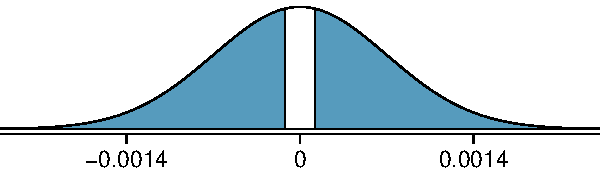
\includegraphics[width=0.6\textwidth]{ch_inference_for_props_oi_biostat/figures/mammograms/mammogramPValue}
\end{center}	
	
Evaluating medical treatments typically requires accounting for evidence that cannot be evaluated from a statistical test. For example, if mammograms are much more expensive than a standard screening and do not offer clear benefits, there is reason to recommend standard screenings over mammograms. Additionally, this study found that mammograms led to overdiagnosis of breast cancer, with some cancers not necessarily causing symptoms during a patient's lifetime; some patients may have been treated unnecessarily. 
	
\end{example}

\index{data!breast cancer|)}
\index{data!mammography|)}

%JV: Commenting out these sections because I want to get to the contigency table method.

\begin{comment}

\subsection{More on 2-proportion hypothesis tests (special topic)}

When we conduct a 2-proportion hypothesis test, usually $H_0$ is $p_1 - p_2 = 0$. However, there are rare situations where we want to check for some difference in $p_1$ and $p_2$ that is some value other than 0. For example, maybe we care about checking a null hypothesis where $p_1 - p_2 = 0.1$.\footnote{We can also encounter a similar situation with a difference of two means, though no such example was given in Chapter~\ref{inferenceForNumericalData} since the methods remain exactly the same in the context of sample means. On the other hand, the success-failure condition and the calculation of the standard error vary slightly in different proportion contexts.} In contexts like these, we generally use $\hat{p}_1$ and $\hat{p}_2$ to check the success-failure condition and construct the standard error.

\begin{exercise}\label{carWheelBladeManufacturer}
A quadcopter company is considering a new manufacturer for rotor blades. The new manufacturer would be more expensive but their higher-quality blades are more reliable, resulting in happier customers and fewer warranty claims. However, management must be convinced that the more expensive blades are worth the conversion before they approve the switch. If there is strong evidence of a more than 3\% improvement in the percent of blades that pass inspection, management says they will switch suppliers, otherwise they will maintain the current supplier. Set up appropriate hypotheses for the test.\footnote{$H_0$: The higher-quality blades will pass inspection just 3\% more frequently than the standard-quality blades. $p_{highQ} - p_{standard} = 0.03$. $H_A$: The higher-quality blades will pass inspection $>$3\% more often than the standard-quality blades. $p_{highQ} - p_{standard} > 0.03$.}
\end{exercise}

\setlength{\captionwidth}{85mm}

\begin{figure}
\centering
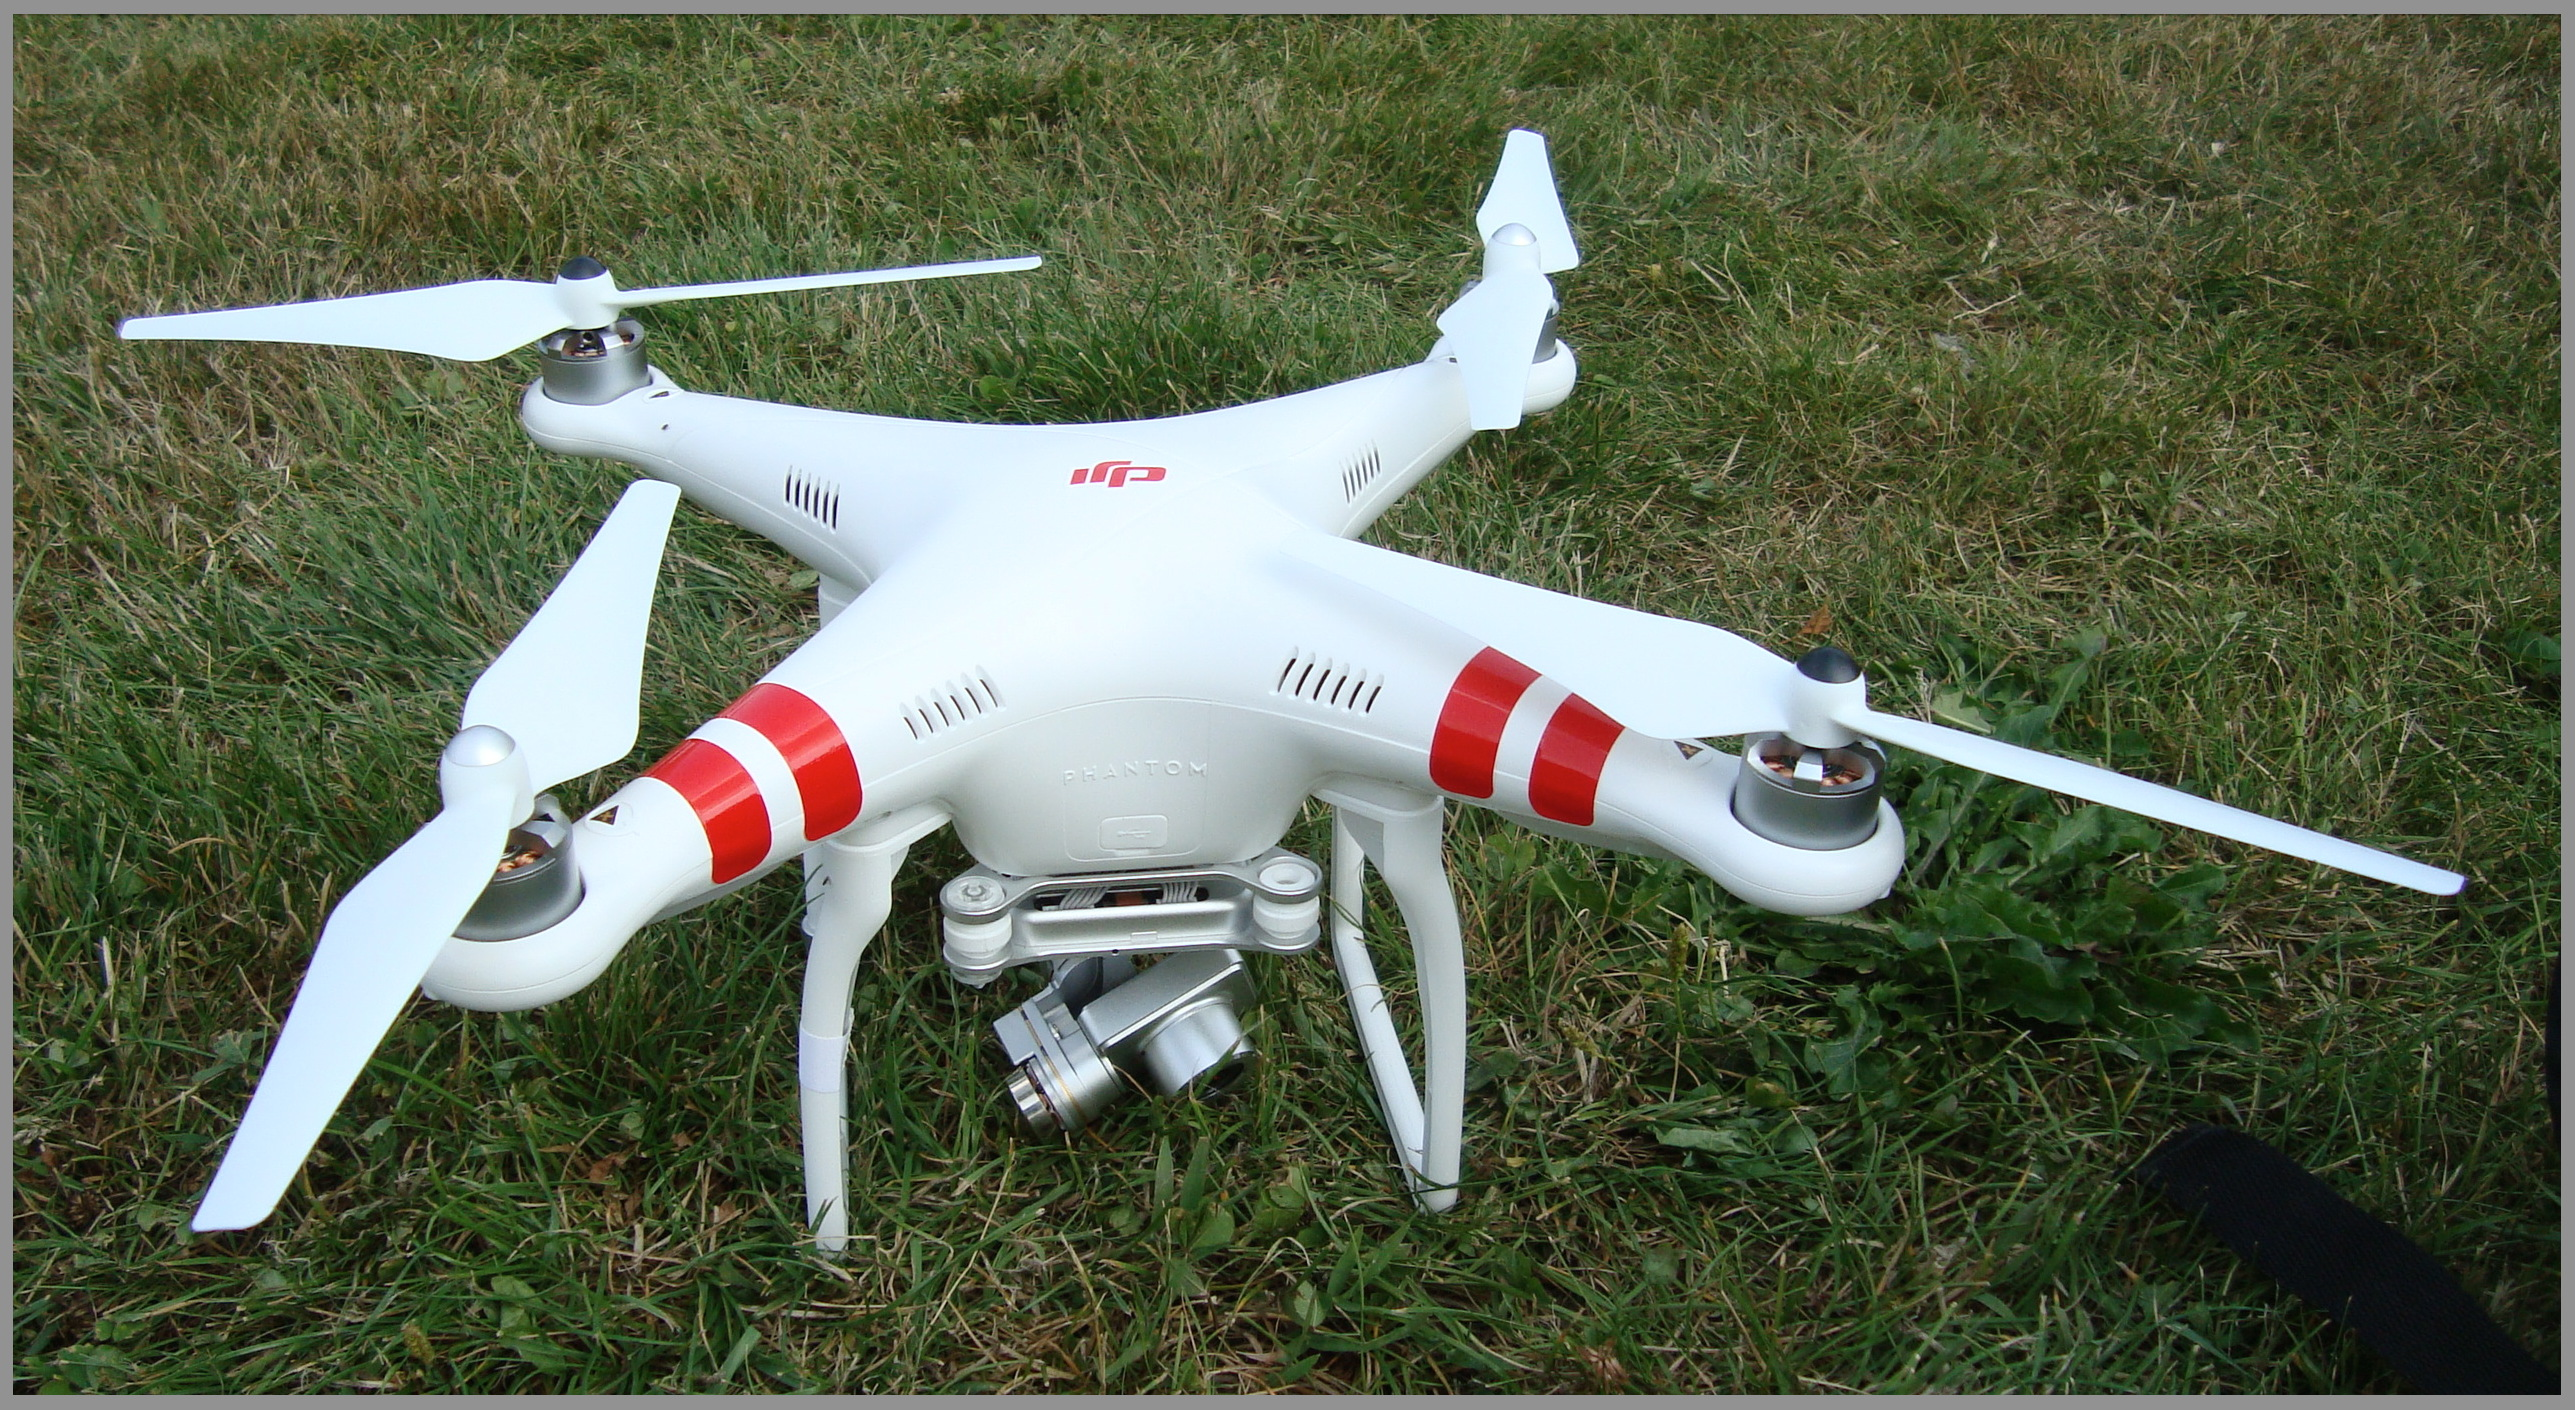
\includegraphics[width=0.6\textwidth]{ch_inference_for_props_oi_biostat/figures/quadcopter/quadcopter_david_j}
\caption{A Phantom quadcopter.\vspace{-1mm} \\
   -----------------------------\vspace{-2mm}\\
   {\footnotesize Photo by David J (\oiRedirect{textbook-quadcopter_david_j}{http://flic.kr/p/oiWLNu}). \oiRedirect{textbook-CC_BY_2}{CC-BY 2.0 license.} This photo has been cropped and a border has been added.}}
\label{quadcopter_david_j}
\end{figure}

\setlength{\captionwidth}{\mycaptionwidth}

%\Add{In Guided Practice~\ref{qualityCtrlEngHypothesisEval}, the null difference is 0.03. However, in the vast majority of applications for differences in means or proportions, the null difference is~0. While the details for a difference of means does not change if the null difference is zero or non-zero, that is not the case for a difference in proportions. As we'll see in Section~\ref{}, a hypothesis test for a difference in proportions where the null value is 0 requires additional~care.}

\begin{example}{The quality control engineer from Guided Practice~\ref{carWheelBladeManufacturer} collects a sample of blades, examining 1000 blades from each company and finds that 899 blades pass inspection from the current supplier and 958 pass inspection from the prospective supplier. Using these data, evaluate the hypothesis setup of Guided Practice~\ref{carWheelBladeManufacturer} with a significance level of 5\%.}\label{qualityCtrlEngHypothesisEval}
First, we check the conditions. The sample is not necessarily random, so to proceed we must assume the blades are all independent; for this sample we will suppose this assumption is reasonable, but the engineer would be more knowledgeable as to whether this assumption is appropriate. The success-failure condition also holds for each sample. Thus, the difference in sample proportions, $0.958 - 0.899 = 0.059$, can be said to come from a nearly normal distribution.

The standard error is computed using the two sample proportions since we do not use a pooled proportion for this context:
\begin{align*}
SE = \sqrt{\frac{0.958(1-0.958)}{1000} + \frac{0.899(1-0.899)}{1000}} = 0.0114
\end{align*}
In this hypothesis test, because the null is that $p_1 - p_2 = 0.03$, the sample proportions were used for the standard error calculation rather than a pooled proportion.

Next, we compute the test statistic and use it to find the p-value, which is depicted in Figure~\ref{bladesTwoSampleHTPValueQC}.
$$Z = \frac{\text{point estimate} - \text{null value}}{SE} = \frac{0.059 - 0.03}{0.0114} = 2.54$$
Using the normal model for this test statistic, we identify the right tail area as 0.006. Since this is a one-sided test, this single tail area is also the p-value, and we reject the null hypothesis because 0.006 is less than 0.05. That is, we have statistically significant evidence that the higher-quality blades actually do pass inspection more than 3\% as often as the currently used blades. Based on these results, management will approve the switch to the new supplier.
\end{example}

\begin{figure}
\centering
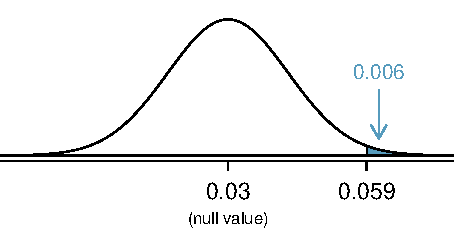
\includegraphics[width=0.5\textwidth]{ch_inference_for_props_oi_biostat/figures/bladesTwoSampleHTPValueQC/bladesTwoSampleHTPValueQC}
\caption{Distribution of the test statistic if the null hypothesis was true. The p-value is represented by the shaded area.}
\label{bladesTwoSampleHTPValueQC}
\end{figure}



%%__________________
%\section{Determining a sample size for an experiment}
%\label{SampleSizeFor2Proportions}
%
%So far we've been focused on controlling the Type~1 Error rate for hypothesis tests. However, when planning an experiment, we often are interested in determining if there is an effect.\footnote{Similar planning is also appropriate for a} There are often two competing considerations:
%\begin{itemize}
%\setlength{\itemsep}{0mm}
%\item We want to collect enough data that we can detect important effects.
%\item In many contexts, collecting data is expensive, so we don't want to collect more than what we need to detect effects we care about.
%\end{itemize}
%The first point is relatively simple: the more data we collect, the more precise our estimates will be, and so we'll be able to detect smaller effects. The second point is more subtle, since we need to determine the size of effects that we care about.
%
%%\begin{example}{Alzheimer's disease is a neurological disease. It affects patients mildly at the beginning and eventually leads to dementia. If an Alzheimer's patient lives long enough, the disease will begin affecting bodily functions and ultimately lead to death. It's an extremely serious condition that millions of people, has no cure, and is very expensive to research, partially due to its slow progression. A group of researchers is }
%\begin{example}{}
%
%\end{example}
%
%
%, even large ones, are difficult to detect with small samples, so we should want to collect a larger sample to detect such effects. If we take a very large sample, we might find a statistically significant difference but the magnitude might be so small that it is of no practical value. In this section we describe techniques for selecting an appropriate sample size based on these considerations.

\end{comment}

%__________________
\section{Inference for two or more groups}
\label{twoWayTablesAndChiSquare}
The comparison of breast cancer death rates between the two groups can also be approached using a two-way contingency table, which contains counts for combinations of outcomes for two variables. The results for the mammogram study in this format are shown in Table~\ref{mammogramStudySummaryTableWithTotals}.

Previously, the main question of interest was stated as, "Is there evidence of a difference in breast cancer death rates between the two screening groups?" If there is no difference in breast cancer death rate by screening method, then screening method and outcome are independent. Thus, the question can be re-phrased: "Is there evidence that screening method is associated with outcome?"

Hypothesis testing in a two-way table assesses whether the two variables of interest are associated (i.e., not independent). This approach is applicable to settings with two or more groups and for responses that have two or more categories. The observed number of counts in each table are compared to the \term{expected} counts if the null hypothesis of association is true; a $\chi^2$ test of significance can then be conducted based on the standardized differences between observed and expected values in each table cell.

\begin{table}[h]
	\centering
	\begin{tabular}{l| l l l l |l}
		\hline
		Death from BC & \hspace{1mm}  & Yes & No & \hspace{1mm} & Total \\
		\hline
		Mammogram				   &    & 500 & 44,425 & 				&44,925 \\
		Control				   &     & 505	& 44,405    &				& 44,910 \\
		\hline
		Total						   &    & 1,005 & 88,830 & 				& 89,835 \\
		\hline
	\end{tabular}
	\caption{Results of the mammogram study, as a contingency table with marginal totals.}
	\label{mammogramStudySummaryTableWithTotals}
\end{table}

\begin{exercise}Formulate hypotheses for a contingency-table approach to analyzing the mammogram data.\footnote{$H_0$: There is no association between type of breast cancer screening and death from breast cancer. $H_A$: There is an association between type of breast cancer screening and death from breast cancer.}

\end{exercise}

\subsection{Expected counts}

If type of breast cancer screening had no effect on outcome in the mammogram data, what would the expected results be? 

Recall that if two events $A$ and $B$ are independent, then $P(A \cap B) = P(A) \times P(B)$. Let $A$ represent assignment to the mammogram group and $B$ represent the event of death from breast cancer. Under independence, the number of individuals out of 89,835 that are expected to be in the mammogram screening group and die from breast cancer equals:

\[89,835 \times P(A)P(B) = 89,835 \times  \frac{44,925}{89,835} \times \frac{1,005}{89,835} = 502.6 \]

Note that the quantities 44,925 and 1,005 are the row and column totals corresponding to the upper left cell of Table~\ref{mammogramStudySummaryTableWithTotals}, where 89,835 is the total number $n$ of observations in the table. A general formula for computing expected counts for any cell can be written from the marginal totals and the total number of observations.

\begin{termBox}{\tBoxTitle{Computing expected counts in a two-way table}
		To identify the expected count for the $i^{th}$ row and $j^{th}$ column, compute
		$$\text{Expected Count}_{\text{row }i,\text{ col }j} = \frac{(\text{row $i$ total}) \times  (\text{column $j$ total})}{\text{table total}}\vspace{2mm}$$}
\end{termBox}	
	
\begin{example}{Calculate expected counts for the data in Table~\ref{mammogramStudySummaryTableWithTotals}.}

	
\[E_{1,1} = \dfrac{44,925 \times 1,005}{89,835} = 502.6 \qquad E_{1,2} = \dfrac{44,925 \times 88,830}{89,835} = 44,422.4\]
\[E_{2,1} = \dfrac{2,922 \times 1,005}{89,835} = 502.4 \qquad E_{2,2} = \dfrac{7,078 \times 88,830}{89,835} = 44,407.6\]
	
\begin{table}[h]
	\centering
		\begin{tabular}{l| l l l l| l}
			\hline
			Death from BC & \hspace{1mm}  & Yes & No & \hspace{1mm} & Total \\
			\hline
			Mammogram				   &    & 500 \highlightO{(502.6)} & 44,425  \highlightO{(44,422.4)} & 				&44,925 \\
			Control				   &     & 505  \highlightO{(502.4)}	& 44,405  \highlightO{(44,407.6)}  &				& 44,910 \\
			\hline
			Total						   &    & 1,005 & 88,830 & 				& 89,835 \\
			\hline
		\end{tabular}
	\caption{Results of the mammogram study, with \highlightO{(expected counts)}. The expected counts should also sum to the row and column totals; this can be a useful check for accuracy.}
	\label{mammogramStudyExpectedCounts}
\end{table}	
	
\end{example}

\begin{example} {If a child is HIV$^+$, should they be treated with nevirapine (NVP) or a more expensive drug, lopinarvir (LPV)? In this setting, success means preventing virologic failure; i.e., growth of the virus. A randomized study was conducted to assess whether there is an association between treatment and outcome. Of the 147 children administered NVP, about 41\% experienced virologic failure; of the 140 children administered LPV, about 19\% experienced virologic failure. Construct a table of observed counts and a table of expected counts.}
	
Convert the proportions to count data: 41\% of 147 is approximately 60, and 19\% of 140 is approximately 27. 

\begin{table}[h]
	\centering
	\begin{tabular}{l | l l | l}
	\hline
	& NVP & LPV & Total \\
	\hline
	Virologic Failure & 60 & 27 & 87 \\
	Stable Disease & 87 & 113 & 200 \\	
	\hline
	Total & 147 & 140 & 287 \\
	\hline
	\end{tabular}
	\caption{Observed counts for the HIV study}
\end{table}

Calculate the expected counts for each cell:

\[E_{1, 1} = \dfrac{87 \times 147}{287} = 44.6 \qquad E_{1, 2} = \dfrac{87 \times 140}{287} = 42.4 \]
\[E_{2, 1} = \dfrac{200 \times 147}{287} = 102.4 \qquad E_{2, 2} = \dfrac{200 \times 140}{287} = 97.6 \]

\begin{table}[h]
	\centering
	\begin{tabular}{l | l l | l}
		\hline
		& NVP & LPV & Total \\
		\hline
		Virologic Failure & 44.6 & 42.4 & 87 \\
		Stable Disease & 102.4 & 97.6 & 200 \\
		\hline	
		Total & 147 & 140 & 287 \\
		\hline
	\end{tabular}
	\caption{Expected counts for the HIV study}
\end{table}

\end{example}

\subsection{The $\chi^2$ test statistic}

Previously, test statistics have been constructed by calculating the difference between a point estimate and a null value, then dividing by the standard error of the point estimate to standardize the difference. Similar logic can be applied in this context to construct a single test statistic, the $\chi^2$ statistic, that measures whether all the standardized differences (one for each cell) are significantly far from zero. If $\chi^2$ is large, this represents a large amount of deviation between the observed and expected values, which suggests evidence against independence of the two variables. The $\chi^2$ test statistic\marginpar[\raggedright\vspace{9mm}

$\chi^2$\vspace{0.5mm}\\\footnotesize chi-square\\test statistic]{\raggedright\vspace{9mm}
	
	$\chi^2$\vspace{0.5mm}\\\footnotesize chi-square\\test statistic}\index{chi-square statistic} is calculated as:

\[\chi^2 = \sum_{\text{all cells}} \frac{(\text{observed} - \text{expected})^2}{\text{expected}} \]

The standardized difference for each cell is a standard normal random variable $Z$. The $\chi^2$ statistic is the sum of squared standard normals; i.e., $\chi^2 = Z_1^2 + Z_2^2 + Z_3^2 + Z_4^2$ for a table with four cells. Squaring each difference allows the $\chi^2$ value to represent the absolute magnitude of how far an observed count differs from an expected count.

It is valid to apply the $\chi^2$ test when 1) each case in a table is independent of the other cases, and 2) each expected cell count is at least 10. The calculations for checking that expected cell counts are at least 10 are identical to those for checking the success-failure condition when conducting a hypothesis test for $p_1 - p_2$:  $n_1 \hat{p} \geq 10$ and $n_2 \hat{p} \geq 10$. This condition ensures that the normal approximation to the binomial can be used.

For example, refer to the mammogram data; the expected counts found in Example~\ref{mammogramStudyExpectedCounts} are identical to the values obtained from checking the success-failure condition in Example~\ref{mammogramSuccessFailure}. Recall that the pooled proportion $\hat{p}$ is the total number of successes $x$ over the total number of cases $n$: $\hat{p} = \frac{x_1 + x_2}{n_1 + n_2}$. In the mammogram table, if "success" is defined as death from breast cancer, then $\hat{p}$ is equal to the (left) column total divided by the total number of cases. The value $n_1$ is the row total of individuals in the mammogram group. Thus, $n_1 \hat{p}  = \frac{\text{(row 1 total) } \times \text{ (col 1 total)}}{\text{table total}}$. The same structure applies for $n_1 (1 - \hat{p})$, $n_2 \hat{p}$, and $n_2 (1 - \hat{p})$.

\begin{termBox}{\tBoxTitle{Conditions for the $\chi^2$ test}
There are two conditions that must be checked before performing a $\chi^2$ test:\vspace{-1mm}
\begin{description}
\setlength{\itemsep}{0mm}
	\item[Independence.] Each case that contributes a count to the table must be independent of all the other cases in the table.
	\item[Sample size.] Each expected cell count must be greater than or equal to 10. For tables larger than $2 \times 2$, it is appropriate to use the test if no more than 1/5 of the expected counts are less than 5, and all expected counts are greater than 1.\footnote{This criterion for large tables is from Rosner's advice on the general $r \times c$ case, pg. 393 of the 7$^{th}$ edition.}
\vspace{-1mm}
\end{description}
}
\end{termBox}


\begin{example}{For the mammogram data, check the conditions for the $\chi^2$ test and calculate the $\chi^2$ test statistic.}

Independence is a reasonable assumption, since individuals have been randomized to either the treatment or control group. Each expected cell count is greater than 10.
\begin{align*}
\chi^2 &= \sum_{\text{all cells}} \frac{(\text{observed} - \text{expected})^2}{\text{expected}} \\
&= \dfrac{(500 - 502.6)^2}{502.6} + \dfrac{(44,425 - 44,422.4)^2}{44,422.4} + \dfrac{(505 - 502.4)^2}{502.4} + \dfrac{(44,405 - 44,407.6)^2}{44,407.6} \\
&=0.02
\end{align*}	
	
\end{example}

\begin{exercise} For the HIV data, check the conditions for the $\chi^2$ test and calculate the $\chi^2$ test statistic.\footnote{Independence holds, since this is a randomized study. The expected counts are greater than 10. $\chi^2 = \frac{(60-44.6)^2}{44.6} + \frac{(27-42.4)^2}{42.4} + \frac{(87-102.4)^2}{102.4} + \frac{(113-97.6)^2}{97.6} = 14.7.$}
	
\end{exercise}

\subsection{Calculating $p$-values for a $\chi^2$ distribution}

The \term{chi-square distribution} is used to characterize data and statistics that are always positive and typically right-skewed. Figure~\ref{chiSquareDistributionWithInceasingDF} demonstrates three general properties of chi-square distributions as the degrees of freedom increases: the distribution becomes more symmetric, the center moves to the right, and the variability inflates.

The $\chi^2$ statistic has a sampling distribution that approximately follows a $\chi^2$ distribution with degrees of freedom $df = (r-1)(c-1)$, where $r$ is the number of rows and $c$ is the number of columns.

\begin{figure}[h]
	\centering
	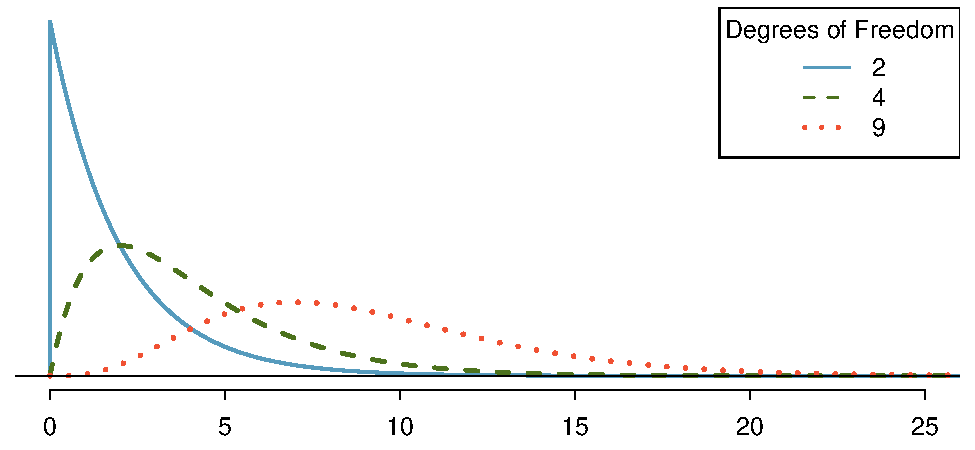
\includegraphics[width=0.9\textwidth]{ch_inference_for_props_oi_biostat/figures/chiSquareDistributionWithInceasingDF/chiSquareDistributionWithInceasingDF}
	\caption{Three chi-square distributions with varying degrees of freedom.}
	\label{chiSquareDistributionWithInceasingDF}
\end{figure}

Either statistical software or a table can be used to calculate $p$-values from the $\chi^2$ distribution. The \term{chi-square table} is partially shown in Table~\ref{chiSquareProbabilityTableShort}, and a more complete table is presented in Appendix~\vref{chiSquareProbabilityTable}. This table is very similar to the $t$-table: each row provides values for distributions with different degrees of freedom, and a cut-off value is provided for specified tail areas. One important difference from the $t$-table is that the $\chi^2$ table only provides upper tail values.

\begin{table}[h]
	\centering
	\begin{tabular}{r | rrrr | rrrr |}
		\hline
		Upper tail & 0.3 & 0.2 & 0.1 & 0.05 & 0.02 & 0.01 & 0.005 & 0.001 \\ 
		\hline
		df \hfill 1 & \footnotesize 1.07 & \footnotesize 1.64 & \footnotesize 2.71 & \footnotesize 3.84 & \footnotesize 5.41 & \footnotesize 6.63 & \footnotesize 7.88 & \footnotesize 10.83 \\ 
		\hfill 2 & \footnotesize 2.41 & \footnotesize 3.22 & \footnotesize 4.61 & \footnotesize 5.99 & \footnotesize 7.82 & \footnotesize 9.21 & \footnotesize 10.60 & \footnotesize 13.82 \\ 
		3 & \footnotesize 3.66 & \footnotesize 4.64 & \footnotesize 6.25 & \footnotesize 7.81 & \footnotesize 9.84 & \footnotesize 11.34 & \footnotesize 12.84 & \footnotesize 16.27 \\ 
		4 & \footnotesize 4.88 & \footnotesize 5.99 & \footnotesize 7.78 & \footnotesize 9.49 & \footnotesize 11.67 & \footnotesize 13.28 & \footnotesize 14.86 & \footnotesize 18.47 \\ 
		5 & \footnotesize 6.06 & \footnotesize 7.29 & \footnotesize 9.24 & \footnotesize 11.07 & \footnotesize 13.39 & \footnotesize 15.09 & \footnotesize 16.75 & \footnotesize 20.52 \\ 
		\hline
		6 & \footnotesize 7.23 & \footnotesize 8.56 & \footnotesize 10.64 & \footnotesize 12.59 & \footnotesize 15.03 & \footnotesize 16.81 & \footnotesize 18.55 & \footnotesize 22.46 \\ 
		7 & \footnotesize 8.38 & \footnotesize 9.80 & \footnotesize 12.02 & \footnotesize 14.07 & \footnotesize 16.62 & \footnotesize 18.48 & \footnotesize 20.28 & \footnotesize 24.32 \\ 
		\hline
	\end{tabular}
	\caption{A section of the chi-square table. A complete table is in Appendix~\vref{chiSquareProbabilityTable}.}
	\label{chiSquareProbabilityTableShort}
\end{table}

\begin{example}{Calculate an approximate $p$-value for the mammogram data, given that the $\chi^2$ statistic equals 0.02. Assess whether the data provides convincing evidence of an association between screening group and breast cancer death.}

The degrees of freedom in a $2 \times 2$ table is 1, so refer to the values in the first column of the probability table. The value 0.02 is less than 1.07, so the $p$-value is greater than 0.3. The data do not provide convincing evidence of an association between screening group and breast cancer death. This supports the conclusions from Example~\ref{mammogramExProp}, where the $p$-value was calculated to be 0.8650.

\begin{figure}[h]
	\centering
	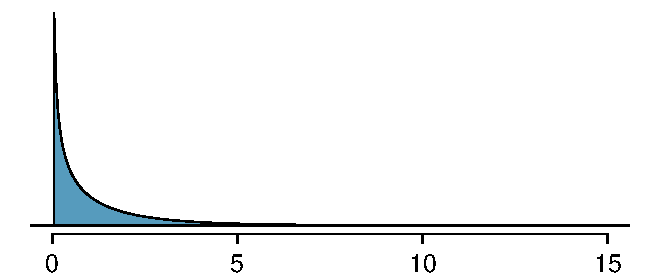
\includegraphics[width=0.55\textwidth]{ch_inference_for_props_oi_biostat/figures/mammogramPValue/mammogramPValue}
	\caption{The $p$-value for the mammogram data is shaded on the $\chi^2$ distribution with $df=1$.}
	\label{mammogramPValue}
\end{figure}

%JV: This figure uses a workaround from the code used to generate the chi-square image for the appendix, but perhaps worth asking where the OI custom function ChiSquareTail is...

\end{example}

\begin{exercise} Calculate an approximate $p$-value for the HIV data. Assess whether the data provides convincing evidence of an association between treatment and outcome at the $\alpha = 0.01$ significance level.\footnote{The $\chi^2$ statistic is 14.7. For degrees of freedom 1, the tail area beyond 14.7 is smaller than 0.001. There is evidence to suggest that treatment is not independent of outcome.}
\label{hivDataPValue}	
\end{exercise}

\subsection{Interpreting the results of a $\chi^2$ test}

If the $p$-value from a $\chi^2$ test is small enough to represent sufficient evidence to reject the null hypothesis, it is important to explore the results further in order to make a complete conclusion about the direction of the observed association. This is done by comparing the observed and expected counts, or by calculating \term{residuals}, which may help in identifying the cells that exhibit the largest discrepancies between observed and expected counts. Calculating residuals can be particularly helpful for understanding the results from large tables.

For each cell in a table, the residual equals:
\[\dfrac{\text{observed} - \text{expected}}{\sqrt{\text{expected}}} \]

Residuals with a large magnitude contribute the most to the $\chi^2$ statistic. If a residual is positive, the observed value is greater than the expected value, and vice versa for a negative residual.

\begin{example}{In the FAMuSS study introduced in Chapter~\ref{introductionToData}, researchers measured a variety of demographic and genetic characteristics for about 1,300 participants, including data on race and genotype at a specific locus on the ACTN3 gene. Is there evidence of an association between genotype and race?
		% latex table generated in R 3.2.4 by xtable 1.8-2 package
		% Wed Dec 07 22:13:57 2016
		\begin{table}[ht]
			\centering
			\begin{tabular}{r | l l l | l}
				\hline
				& CC & CT & TT & Sum \\ 
				\hline
				African American & 16 & 6 & 5 & 27 \\ 
				Asian & 21 & 18 & 16 & 55 \\ 
				Caucasian & 125 & 216 & 126 & 467 \\ 
				Hispanic & 4 & 10 & 9 & 23 \\ 
				Other & 7 & 11 & 5 & 23 \\ 
				\hline
				Sum & 173 & 261 & 161 & 595 \\ 
				\hline
			\end{tabular}
			\caption{Observed counts for race and genotype data from the FAMuSS study.}
		\end{table}
		%labels modified from xtable
	}	
	
First, check the assumptions for applying a $\chi^2$ test. It is reasonable to assume independence, since it is unlikely that any participants were related to each other. None of the expected counts, as shown in Table~\ref{famussExpected}, are less than 5.

% latex table generated in R 3.2.4 by xtable 1.8-2 package
% Thu Dec 08 10:34:51 2016
\begin{table}[ht]
	\centering
	\begin{tabular}{r| l l l | l}
		\hline
		& CC & CT & TT & Sum \\ 
		\hline
		African Am & 7.85 & 11.84 & 7.31 & 27.00 \\ 
		Asian & 15.99 & 24.13 & 14.88 & 55.00 \\ 
		Caucasian & 135.78 & 204.85 & 126.36 & 467.00 \\ 
		Hispanic & 6.69 & 10.09 & 6.22 & 23.00 \\ 
		Other & 6.69 & 10.09 & 6.22 & 23.00 \\ 
		\hline
		Sum & 173.00 & 261.00 & 161.00 & 595.00 \\ 
		\hline
	\end{tabular}
	\caption{Expected counts for race and genotype data from the FAMuSS study.}
	\label{famussExpected}
\end{table}
%labels and formatting modified

$H_0$: Race and genotype are independent.

$H_A$: Race and genotype are not independent.

Let $\alpha = 0.05$.

Calculate the $\chi^2$ statistic:
\begin{align*}
\chi^2 &= \sum_{\text{all cells}} \frac{(\text{observed} - \text{expected})^2}{\text{expected}} \\
&= \dfrac{(16-7.85)^2}{7.85} + \dfrac{(6-11.84)^2}{11.84} + ... + \dfrac{(5 - 6.22)^2}{6.22} \\
&=19.4
\end{align*}	

Calculate the $p$-value: for a table with 3 rows and 5 columns, the $\chi^2$ statistic is distributed with $(3-1)(5-1) = 8$ degrees of freedom. From the table, a $\chi^2$ value of 19.4 corresponds to a tail area between 0.01 and 0.02.\footnote{The exact $p$-value can be obtained from software: $p = 0.013$.} Thus, there is sufficient evidence to reject the null hypothesis of independence between race and genotype.

To further explore the differences in genotype distribution between races, calculate residuals for each cell. The largest residuals are in the first row; there are many more African Americans with the CC genotype than expected under independence, and fewer with the CT genotype than expected. The residuals in the second row indicate a similar trend for Asians, but with a less pronounced difference. These results suggest further directions for research; a future study could enroll a larger number of African American and Asian participants to examine whether the observed trend holds with a more representative sample. Geneticists might also be interested in exploring whether this genetic difference between populations has an observable phenotypic effect.

% latex table generated in R 3.2.4 by xtable 1.8-2 package
% Thu Dec 08 10:48:57 2016
\begin{table}[ht]
	\centering
	\begin{tabular}{r|lll|l}
		\hline
		& CC & CT & TT & Sum \\ 
		\hline
		African Am & \highlightO{2.91} & \highlightO{-1.70} & -0.85 & 0.00 \\ 
		Asian & \highlightO{1.25} & \highlightO{-1.25} & 0.29 & 0.00 \\ 
		Caucasian & -0.93 & 0.78 & -0.03 & 0.00 \\ 
		Hispanic & -1.04 & -0.03 & 1.11 & 0.00 \\ 
		Other & 0.12 & 0.29 & -0.49 & 0.00 \\ 
		\hline
		Sum & 0.00 & 0.00 & 0.00 & 0.00 \\ 
		\hline
	\end{tabular}
	\caption{Residuals for race and genotype data from the FAMuSS study}
\end{table}
	
\end{example}

\begin{example}{In Guided Practice~\ref{hivDataPValue}, the $p$-value was found to be smaller than 0.001, suggesting that treatment is not independent of outcome. Does the evidence suggest that infants should be given nevirapine or lopinarvir?

\begin{table}[h]
	\centering
	\begin{tabular}{l | l l | l}
		\hline
		& NVP & LPV & Total \\
		\hline
		Virologic Failure & 60 \highlightO{44.6} & 27 \highlightO{42.4} & 87 \\
		Stable Disease & 87 \highlightO{102.4} & 113 \highlightO{97.6}& 200 \\	
		\hline
		Total & 147 & 140 & 287 \\
		\hline
	\end{tabular}
	\caption{Observed and \highlightO{(expected)} counts for the HIV study.}
\end{table}			
		
} 
	
In a $2 \times 2$ table, it is relatively easy to directly compare observed and expected counts. 

For nevirapine, more infants than expected experienced virologic failure (60 > 44.6), while fewer than expected reached a stable disease state (87 < 102.4). For lopinarvir, fewer infants than expected experienced virologic failure (27 < 42.4), and more infants than expected reached a stable disease state (113 > 97.6). The outcomes for infants on lopinarvir are better than for those on nevirapine; combined with the results of the significance test, the data suggest that lopinarvir is associated with better treatment outcomes.
\label{HIVDirectionEx}	
\end{example}

\begin{exercise} Confirm the conclusions reached in Example~\ref{HIVDirectionEx} by analyzing the residuals.\footnote{$R_{1, 1} = \frac{(44.6-60)}{\sqrt{44.6}} = 2.31$; $R_{1, 2} = \frac{(42.4-27)}{\sqrt{27}} = -2.37$; $R_{2, 1} = \frac{(87-102.4)}{\sqrt{102.4}} = -1.53$; $R_{2, 2} = \frac{(113-97.6)}{\sqrt{97.6}} = 1.56$. The positive residuals for the upper left and lower right cells indicate that more infants than expected experienced virologic failure on NVP and stable disease on LPV; vice versa for the upper right and lower left cells. The larger magnitude of the residuals for the two NVP cells indicates that most of the discrepancy between observed and expected counts is for outcomes related to NVP.}
\end{exercise}

\begin{exercise} Chapter~\ref{introductionToData} started with the discussion of a study examining whether exposure to peanut products reduce the rate of a child developing peanut allergies. Children were randomized either to the peanut avoidance or the peanut consumption group; at 5 years of age, each child was tested for peanut allergy using an oral food challenge (OFC). The results of the OFC are reproduced in Table~\ref{leapStudyResultsTest}; failing the food challenge indicates an allergic reaction. Assess whether there is evidence for exposure to peanut allergy reducing the chance of developing peanut allergies.\footnote{The assumptions for conducting a $\chi^2$ test are satisfied. Calculate a $\chi^2$ test statistic: 24.29. The associated $p$-value is $8.3 \times 10^{-7}$. There is evidence to suggest that treatment group is not independent of outcome. Specifically, a residual analysis shows that in the peanut avoidance group, more children than expected failed the OFC; in the peanut consumption group, more children than expected passed the OFC.}
	
	% latex table generated in R 3.1.1 by xtable 1.7-4 package
	% Thu Jul 16 07:12:04 2015
	\begin{table}[h]
		\centering
		\begin{tabular}{rrrr}
			\hline
			& FAIL OFC & PASS OFC & Sum \\ 
			\hline
			Peanut Avoidance & 36 & 227 & 263 \\ 
			Peanut Consumption & 5 & 262 & 267 \\ 
			Sum & 41 & 489 & 530 \\ 
			\hline
		\end{tabular}
		\caption{LEAP Study Results} 
		\label{leapStudyResultsTest}
	\end{table}
	%library(xtable); outcome.table = addmargins(table(LEAP$treatment.group, LEAP$overall.V60.outcome)); xtable(outcome.table, digits = 0, caption = "LEAP Study Results", caption  = "leapStudyResults")
	
	
\end{exercise}

\subsection{Fisher's exact test}

If sample sizes are too small, it is not valid to assess independence with the $\chi^2$ test. When expected counts in a table are less than 5, \term{Fisher's exact test} can be used to calculate exact levels of significance. This test is usually applied to $2 \times 2$ tables. Although it is possible to use the test on larger tables, the calculations involved are computationally intensive, and software packages will typically use simulation methods instead. 

\textit{Clostridium difficile} is a bacterium that causes inflammation of the colon. Antibiotic treatment is typically not effective, particularly for patients that experience multiple recurrences of infection. Infusion of feces from healthy donors has been reported as an effective treatment for recurrent infection. A randomized trial was conducted to compare the efficacy of donor-feces infusion versus vancomycin, the antibiotic typically prescribed to treat \textit{C. difficile }infection. The results of the trial are shown in Table~\ref{fecalStudyResultsTest}.\footnote{These results correspond to the number of patients cured after the first infusion of donor feces and the number of patients cured in the vancomycin-alone group.} The expected values of this table are too small for the $\chi^2$ method to be valid.

%JV: Expected values are 9.3, 6.6, 7.6, 5.4. Need to adjust depending on value decided for using normal approximation.

Under the null hypothesis, the cure rates for the fecal infusion and fecal infusion groups are equal; i.e., individuals in one group are just as likely to be cured as individuals in the other group. Suppose the probability that an individual is cured given they were assigned to the fecal infusion group is $p_1$ and the probability an individual is cured given they were assigned to the vancomycin group is $p_2$. Researchers are interested in testing the null hypothesis $H_0$: $p_1 = p_2$.

%data from \medicine\feces_infusion

\begin{table}[h]
	\centering
	\begin{tabular}{rrrr}
		\hline
		& Cured & Uncured & Sum \\ 
		\hline
		Fecal Infusion & 13 & 3 & 16 \\ 
		Vancomycin & 4 & 9 & 13 \\ 
		Sum & 17 & 12 & 29 \\ 
		\hline
	\end{tabular}
	\caption{Fecal Infusion Study Results} 
	\label{fecalStudyResultsTest}
\end{table}

The $p$-value is the probability of observing results as or more extreme than those observed, if the null hypothesis is true. Previously discussed methods for significance testing have relied on calculating a test statistic associated with a defined sampling distribution, then obtaining $p$-values from tail areas on the distribution. 

Fisher's exact test uses a different approach; the $p$-value is calculated by adding together the individual probabilities of obtaining each result that is as or more extreme than those observed, given fixed marginal totals. 

\begin{itemize}
	\item A single result is defined as the unique combination of values in the four main cells when the marginal totals are held constant. If the margins are fixed, any single table can be identified from knowing just one of the values in the table. For example, if the marginal sums in Table~\ref{fecalStudyResultsTest} are known, along with the value in one cell (e.g., the upper right equals 3), it is possible to calculate the values in the other three cells. 
	
	\item Extreme results are defined in relation to the null hypothesis of $p_1 = p_2$. In the fecal infusion data, about $(0.50)(17) = 8.5$ cured patients are expected in each treatment group under the null hypothesis. It would be considered extreme if all 17 cured patients were in the fecal infusion group and 0 in the vancomycin group; an extreme result in the other direction would be, for instance, 1 cured patient in the fecal infusion group and 16 in the vancomycin group.
\end{itemize}

\newpage

\begin{example}{Of the 17 patients cured, 13 were in the fecal infusion group and 4 were in the vancomycin group. Assume that the marginal totals are fixed (i.e., 17 patients were cured, 12 were uncured, and 16 patients were in the fecal infusion group, while 13 were in the vancomycin group). Enumerate all possible sets of results that are more extreme in the same direction than what was observed.}
	
The observed results show a case of $\hat{p}_1 > \hat{p}_2$; results that are more extreme consist of cases where more than 13 cured patients were in the fecal infusion group. Under the assumption that the total number of cured patients is constant at 17 and that only 16 patients were assigned to the fecal infusion group (out of 29 patients total), more extreme results are represented by cases where 14, 15, or 16 cured patients were in the fecal infusion group. The following tables illustrate the unique combinations of values $a, b, c, d$ corresponding to those extreme results.

\begin{table}[h]
	\centering
	\color{gray}
	\begin{tabular}{r|cc|c}
		\hline
		& Cured & Uncured & Sum \\ 
		\hline
		Fecal Infusion & \textcolor{black}{14} & \textcolor{black}{2} & 16 \\ 
		Vancomycin & \textcolor{black}{3} & \textcolor{black}{10} & 13 \\ 
		\hline
		Sum & 17 & 12 & 29 \\ 
		\hline
	\end{tabular}
\end{table}

\begin{table}[h]
	\centering
	\color{gray}
	\begin{tabular}{r|cc|c}
		\hline
		& Cured & Uncured & Sum \\ 
		\hline
		Fecal Infusion & \textcolor{black}{15} & \textcolor{black}{1} & 16 \\ 
		Vancomycin & \textcolor{black}{2} & \textcolor{black}{11} & 13 \\ 
		\hline
		Sum & 17 & 12 & 29 \\ 
		\hline
	\end{tabular}
\end{table}

\begin{table}[h]
	\centering
	\color{gray}
	\begin{tabular}{r|cc|c}
		\hline
		& Cured & Uncured & Sum \\ 
		\hline
		Fecal Infusion & \textcolor{black}{16} & \textcolor{black}{0} & 16 \\ 
		Vancomycin & \textcolor{black}{1} & \textcolor{black}{12} & 13 \\ 
		\hline
		Sum & 17 & 12 & 29 \\ 
		\hline
	\end{tabular}
\end{table}
	
\label{fecalStudyExtreme}	
\end{example}

\subsubsection{Calculating a one-sided $p$-value}

Suppose that researchers were interested in testing the null hypothesis against the one-sided alternative, $H_A: p_1 > p_2$. To calculate the one-sided $p$-value, sum the probabilities of each table representing results as or more extreme than those observed, in the same direction; specifically, sum the probabilities of observing the tables in Example~\ref{fecalStudyExtreme} and of observing Table~\ref{fecalStudyResultsTest}.

\begin{table}[h]
	\centering
	\begin{tabular}{rccc}
		\hline
		& Cured & Uncured & Sum \\ 
		\hline
		Fecal Infusion & $a$ & $b$ & $a+b$ \\ 
		Vancomycin & $c$ & $d$ & $c+d$ \\ 
		Sum & $a+c$ & $b+d$ & $n$ \\ 
		\hline
	\end{tabular}
	\caption{General Layout of Data in Fecal Infusion Study} 
	\label{fecalStudyGeneral}
\end{table}


The probability of observing a table with cells $a, b, c, d$ given fixed marginal totals $a+b$, $c+d$, $a + c$, and $b +d$ follows the hypergeometric distribution.

\[P(a,b,c,d) = \text{HGeom}(a+b, c+d, a+c) = \dfrac{ {a+b \choose a} {c+d \choose c}}{{n \choose a+c}} = \dfrac{(a+b)! \text{ } (c+d)! \text{ } (a+c)! \text{ } (b+d)!}{a! \text{ } b! \text{ } c! \text{ } d! \text{ } n!}\]

\begin{example}{Calculate the probability of observing Table~\ref{fecalStudyResultsTest}, assuming the margin totals are fixed.}

\[P(13, 3, 4, 9) = \dfrac{ {16 \choose 13} {13 \choose 4}}{{29 \choose 17}} = \dfrac{16! \text{ } 13! \text{ } 17! \text{ } 12!}{13! \text{ } 3! \text{ } 4! \text{ } 9! \text{ } 29!} = 7.71 \times 10^{-3}\]

The value .0077 represents the probability of observing 13 cured patients out of 16 individuals in the fecal infusion group, given that there are a total of 29 patients and 17 were cured overall.
\end{example}

\begin{example}{Evaluate the statistical significance of the observed data in Table~\ref{fecalStudyResultsTest} using the one-sided alternative $H_A: p_1 > p_2$.}

Calculate the probability of the tables from Example~\ref{fecalStudyExtreme}. Generally, the formula for these tables is 
\[P(a, b, c, d) = \dfrac{ {a+b \choose a} {c+d \choose c}}{{n \choose a+c}} = \dfrac{ {16 \choose a} {13 \choose c}}{{29 \choose 17}},\] 

since the marginal totals from Table~\ref{fecalStudyResultsTest} are fixed. The value $a$ ranges from 14, 15, 16, while $c$ ranges from 3, 2, 1.
\begin{align*}
P(14, 2, 3, 10) &= \dfrac{ {16 \choose 14} {13 \choose 3}}{{29 \choose 17}} = 6.61 \times 10^{-4} \\
P(15, 1, 2, 11) &= \dfrac{ {16 \choose 15} {13 \choose 2}}{{29 \choose 17}} = 2.40 \times 10^{-5} \\
P(16, 0, 1, 12) &= \dfrac{ {16 \choose 16} {13 \choose 1}}{{29 \choose 17}} = 2.51 \times 10^{-7}
\end{align*}

The probability of the observed table is $7.71 \times 10^{-3}$, as calculated in the previous example.

The one-sided $p$-value is the sum of these table probabilities: $(7.71 \times 10^{-3}) + (6.61 \times 10^{-4}) + (2.40 \times 10^{-5}) + (2.51 \times 10^{-7}) = 0.0084.$

The results are significant at the $\alpha = 0.05$ significance level. There is evidence to support the one-sided alternative that the proportion of cured patients in the fecal infusion group is higher than the proportion of cured patients in the vancomycin group. However, it is important to note that two-sided alternatives are the standard in medical literature. Conducting a two-sided test would be especially desirable when evaluating a treatment which lacks randomized trials supporting its efficacy, such as donor-feces infusion.
\end{example}

\subsubsection{Calculating a two-sided $p$-value}

There are various methods for calculating a two-sided $p$-value in the Fisher's exact test setting. One common method used by various statistical computing packages such as \textsf{R} is to classify "more extreme" tables as all tables with probabilities less than that of the observed table, in both directions. The two-sided $p$-value is the sum of probabilities for the qualifying tables.

\begin{example}{Evaluate the statistical significance of the observed data in Table~\ref{fecalStudyResultsTest} using the two-sided alternative $H_A: p_1 \neq p_2$.}
	
The one-sided $p$-value, calculated from adding extreme tables in the same direction as the observed data, is 0.0084. Identify tables that are more extreme in the other direction, i.e. where the proportion of cured patients in the vancomycin group are higher than in the fecal infusion group. Start with the most extreme cases and calculate probabilities until a table has a $p$-value higher than $7.71 \times 10^{-3}$, the probability of the observed table. 

The most extreme result in the $\hat{p}_1 < \hat{p}_2$ direction would be if all patients in the vancomycin group were cured; then 13 of the cured patients would be in the vancomycin group and 4 would be in the fecal transplant group. This table has probability $3.5 \times 10^{-5}$.

\begin{table}[h]
	\centering
	\color{gray}
	\begin{tabular}{r|cc|c}
		\hline
		& Cured & Uncured & Sum \\ 
		\hline
		Fecal Infusion & \textcolor{black}{4} & \textcolor{black}{12} & 16 \\ 
		Vancomycin & \textcolor{black}{13} & \textcolor{black}{0} & 13 \\ 
		\hline
		Sum & 17 & 12 & 29 \\ 
		\hline
	\end{tabular}
\end{table}

Continue enumerating tables by decreasing the number of cured patients in the vancomycin group. The table with 5 cured patients in the fecal infusion group has probability $1.09 \times 10^{-3}$.

\begin{table}[h]
	\centering
	\color{gray}
	\begin{tabular}{r|cc|c}
		\hline
		& Cured & Uncured & Sum \\ 
		\hline
		Fecal Infusion & \textcolor{black}{5} & \textcolor{black}{11} & 16 \\ 
		Vancomycin & \textcolor{black}{12} & \textcolor{black}{1} & 13 \\ 
		\hline
		Sum & 17 & 12 & 29 \\ 
		\hline
	\end{tabular}
\end{table}

The table with 6 cured patients in the fecal infusion group has probability 0.012. This value is greater than $7.71 \times 10^{-3}$, so it will not be part of the sum to calculate the two-sided $p$-value.
	
\begin{table}[h]
	\centering
	\color{gray}
	\begin{tabular}{r|cc|c}
		\hline
		& Cured & Uncured & Sum \\ 
		\hline
		Fecal Infusion & \textcolor{black}{6} & \textcolor{black}{10} & 16 \\ 
		Vancomycin & \textcolor{black}{11} & \textcolor{black}{2} & 13 \\ 
		\hline
		Sum & 17 & 12 & 29 \\ 
		\hline
	\end{tabular}
\end{table}	

Thus, the two-sided $p$-value for these data equals $0.0084 + (3.5 \times 10^{-5}) + (1.09 \times 10^{-3}) = 0.0095$. The results are significant at the $\alpha = 0.01$ significance level, and there is evidence to support the efficacy of donor-feces infusion as a treatment for recurrent \textit{C. difficile} infection.

\textit{JV: According to Figure 2 of the paper, though, they report a $p$-value of 0.008, which corresponds to the one-sided $p$-value? Results in R agree with the hand calculations.}
	
\end{example}

\textit{JV: Did not look for a good example for a guided practice yet, as the table needs to be relatively small for the hand calculation method to be reasonable.}

%__________________
\section[Testing for goodness of fit using chi-square (special topic)]{Testing for goodness of fit using chi-square \\(special topic)}
\label{oneWayChiSquare}

The $\chi^2$ test can also be used to assess a null model when data for a single variable is sorted across several categories. This technique is commonly used in two circumstances: 1) Given a sample of cases that can be classified into several groups, determine if the sample is representative of the general population, 2) Evaluate whether data resemble a particular distribution. 

As with testing in the two-way table setting, expected counts are calculated based on the assumption that the null hypothesis is true. It is valid to apply the $\chi^2$ distribution when each expected count is at least 5. In this setting, the $\chi^2$ statistic follows a $\chi^2$ distribution with $k-1$ degrees of freedom, where $k$ is the number of categories. 

\begin{example} {It is not clear that the participants in the FAMuSS study are representative of the general United States population. For example, are the participants racially representative of the general population? Assess whether the proportions from each race in the FAMuSS data are indicative of a random sample from the population.
		
The following data are from the U.S. Census Bureau report from 2004, the year that the FAMusSS study was published.\footnote{The US Census Bureau considers Hispanic as a classification separate from race, on the basis that Hispanic individuals can be any race. In order to facilitate the comparison with the FAMuSS data, participants identified as "Hispanic" have been merged with the "Other" category.}

\begin{table}[h]
	\centering
	\begin{tabular}{ll ccc c ll}
		\hline
		Race	 & \hspace{2mm} & African American & Asian & Caucasian & Other & \hspace{2mm} & Total \\
		\hline
		FAMuSS &	& 27 & 55 & 467 & 46 & & 595 \\
		US Census	 & 		& 0.128 & 0.01 & 0.804 & 0.058 & & 1.00 \\
		\hline
	\end{tabular}
	\caption{Representation by race in the FAMuSS study versus the general population.}
\end{table}
		
}

Calculate expected counts under the null hypothesis that the sample proportions should equal the population proportions. For example, since African Americans are 0.128 of the general proportion, $(0.128)(595) = 76.16$ African Americans are expected in the sample.

\begin{table}[h]
	\centering
	\begin{tabular}{ll ccc c ll}
		\hline
		Race	 & \hspace{2mm} & African American & Asian & Caucasian & Other & \hspace{2mm} & Total \\
		\hline
		Observed &	& 27 & 55 & 467 & 46 & & 595 \\
		Expected & 	& 76.16 & 5.95 & 478.38 & 34.51 & & 595 \\
		\hline
	\end{tabular}
	\caption{Actual and expected counts in the FAMuSS data.}
\end{table}	

Each expected count is greater than or equal to 5; proceed with the $\chi^2$ test.
\begin{align*}
\chi^2 &= \sum_{\text{all cells}} \frac{(\text{observed} - \text{expected})^2}{\text{expected}} \\
&= \dfrac{(27-76.16)^2}{76.16} + \dfrac{(55-5.95)^2}{5.95} + \dfrac{(467-478.38)^2}{478.38} + \dfrac{(46-34.51)^2}{34.51} \\
&=440.18
\end{align*}	

There are 3 degrees of freedom, since $k = 4$. The $\chi^2$ statistic is extremely large, and the associated tail area is smaller than 0.001. There is sufficient evidence to reject the null hypothesis that the sample is representative of the general population. A comparison of the observed and expected values (or the residuals) indicates that the largest discrepancy is with the over-representation of Asian participants.
\end{example}

%2004 US Census data: https://www.census.gov/population/pop-profile/dynamic/RACEHO.pdf

\begin{example}{According to Mendelian genetics, alleles segregate independently; if an individual is heterozygous for a gene and has alleles $A$ and $B$, then the alleles have an equal chance of being passed to an offspring. Under this framework, if two individuals with genotype $AB$ mate, then their offspring are expected to exhibit a 1:2:1 genotypic ratio; 25\% of the offspring will be $AA$, 50\% will be $AB$, and 50\% will be $BB$. The term "segregation distortion" refers to a deviation from expected Mendelian frequencies. 
		
At a specific gene locus in the plant \textit{Arabidopsis thaliana}, researchers have observed 84 $AA$ individuals, 233 $AB$ individuals, and 134 $BB$ individuals. Is there evidence of segregation disorder at this locus? Conduct the test at $\alpha = 0.0001$ to account for multiple testing, since the original study examined approximately 250 locations across the genome. 
}

The Mendelian proportions are 25\%, 50\%, and 25\%. Thus, the expected counts in a group of 451 individuals are: 112.75 $AA$, 225.50 $AB$, and 112.75 $BB$. No expected count is less than 5.

\begin{align*}
\chi^2 &= \sum_{\text{all cells}} \frac{(\text{observed} - \text{expected})^2}{\text{expected}} \\
&= \dfrac{(84-112.75)^2}{112.75} + \dfrac{(233-225.50)^2}{225.50} + \dfrac{(134-112.75)^2}{112.75}\\
&=11.59
\end{align*}

There are 2 degrees of freedom, since $k = 2$. The $p$-value is between 0.005 and 0.001, which is greater than $\alpha = 0.0001$. There is insufficient evidence to reject the null hypothesis that the offspring ratios correspond to expected Mendelian frequencies.
\end{example}

\begin{comment}

%__________________
\section[Small sample hypothesis testing for a proportion (special topic)]{Small sample hypothesis testing for a proportion\\(special topic)}
\label{smallSampleHTForProportion}

In this section we develop inferential methods for a single proportion that are appropriate when the sample size is too small to apply the normal model to $\hat{p}$. Just like the methods related to the $t$-distribution, these methods can also be applied to large samples.

\subsection{When the success-failure condition is not met}

\index{data!medical consultant|(}
People providing an organ for donation sometimes seek the help of a special ``medical consultant''. These consultants assist the patient in all aspects of the surgery, with the goal of reducing the possibility of complications during the medical procedure and recovery. Patients might choose a consultant based in part on the historical complication rate of the consultant's clients. One consultant tried to attract patients by noting the average complication rate for liver donor surgeries in the US is about 10\%, but her clients have only had 3 complications in the 62 liver donor surgeries she has facilitated. She claims this is strong evidence that her work meaningfully contributes to reducing complications (and therefore she should be hired!).

\begin{exercise}
We will let $p$ represent the true complication rate for liver donors working with this consultant. Estimate $p$ using the data, and label this value~$\hat{p}$.\footnote{The sample proportion: $\hat{p} = 3/62 = 0.048$}
\end{exercise}

\begin{example}{Is it possible to assess the consultant's claim with the data provided?}
No. The claim is that there is a causal connection, but the data are observational. Patients who hire this medical consultant may have lower complication rates for other reasons.

While it is not possible to assess this causal claim, it is still possible to test for an association using these data. For this question we ask, could the low complication rate of $\hat{p} = 0.048$ be due to chance?
\end{example}

\begin{exercise} \label{hypForAssessingConsultantWorkInLiverTransplants}
Write out hypotheses in both plain and statistical language to test for the association between the consultant's work and the true complication rate, $p$, for this consultant's clients.\footnote{$H_0$: There is no association between the consultant's contributions and the clients' complication rate. In statistical language, $p=0.10$. $H_A$: Patients who work with the consultant tend to have a complication rate lower than 10\%, i.e. $p<0.10$.}
\end{exercise}

\begin{example}{In the examples based on large sample theory, we modeled $\hat{p}$ using the normal distribution. Why is this not appropriate here?}
The independence assumption may be reasonable if each of the surgeries is from a different surgical team. However, the success-failure condition is not satisfied. Under the null hypothesis, we would anticipate seeing $62\times 0.10=6.2$ complications, not the 10 required for the normal approximation.
\end{example}

The uncertainty associated with the sample proportion should not be modeled using the normal distribution. However, we would still like to assess the hypotheses from Guided Practice~\ref{hypForAssessingConsultantWorkInLiverTransplants} in absence of the normal framework. To do so, we need to evaluate the possibility of a sample value ($\hat{p}$) this far below the null value, $p_0=0.10$. This possibility is usually measured with a p-value.

The p-value is computed based on the null distribution, which is the distribution of the test statistic if the null hypothesis is true. Supposing the null hypothesis is true, we can compute the p-value by identifying the chance of observing a test statistic that favors the alternative hypothesis at least as strongly as the observed test statistic. This can be done using simulation.


\subsection{Generating the null distribution and p-value by simulation}
\label{generatingTheNullDistributionAndPValueBySimulationForOneProportion}

We want to identify the sampling distribution of the test statistic ($\hat{p}$) if the null hypothesis was true. In other words, we want to see how the sample proportion changes due to chance alone. Then we plan to use this information to decide whether there is enough evidence to reject the null hypothesis.

Under the null hypothesis, 10\% of liver donors have complications during or after surgery. Suppose this rate was really no different for the consultant's clients. If this was the case, we could \emph{simulate} 62 clients to get a sample proportion for the complication rate from the null distribution.

Each client can be simulated using a deck of cards. Take one red card, nine black cards, and mix them up. Then drawing a card is one way of simulating the chance a patient has a complication \emph{if the true complication rate is 10\%} for the data. If we do this 62 times and compute the proportion of patients with complications in the simulation, $\hat{p}_{sim}$, then this sample proportion is exactly a sample from the null distribution.

An undergraduate student was paid \$2 to complete this simulation. There were 5 simulated cases with a complication and 57 simulated cases without a complication, i.e. $\hat{p}_{sim} = 5/62 = 0.081$.

\begin{example}{Is this one simulation enough to determine whether or not we should reject the null hypothesis from Guided Practice~\ref{hypForAssessingConsultantWorkInLiverTransplants}? Explain.}
No. To assess the hypotheses, we need to see a distribution of many $\hat{p}_{sim}$, not just a \emph{single} draw from this sampling distribution.
\end{example}

One simulation isn't enough to get a sense of the null distribution; many simulation studies are needed. Roughly 10,000 seems sufficient. However, paying someone to simulate 10,000 studies by hand is a waste of time and money. Instead, simulations are typically programmed into a computer, which is much more efficient.

Figure~\ref{nullDistForPHatIfLiverTransplantConsultantIsNotHelpful} shows the results of 10,000 simulated studies. The proportions that are equal to or less than $\hat{p}=0.048$ are shaded. The shaded areas represent sample proportions under the null distribution that provide at least as much evidence as $\hat{p}$ favoring the alternative hypothesis. There were 1222 simulated sample proportions with $\hat{p}_{sim} \leq 0.048$. We use these to construct the null distribution's left-tail area and find the p-value:
\begin{align}
\text{left tail }\label{estOfPValueBasedOnSimulatedNullForSingleProportion}
	&= \frac{\text{Number of observed simulations with }\hat{p}_{sim}\leq\text{ 0.048}}{10000}
\end{align}
Of the 10,000 simulated $\hat{p}_{sim}$, 1222 were equal to or smaller than $\hat{p}$. Since the hypothesis test is one-sided, the estimated p-value is equal to this tail area: 0.1222.
\begin{figure}
\centering
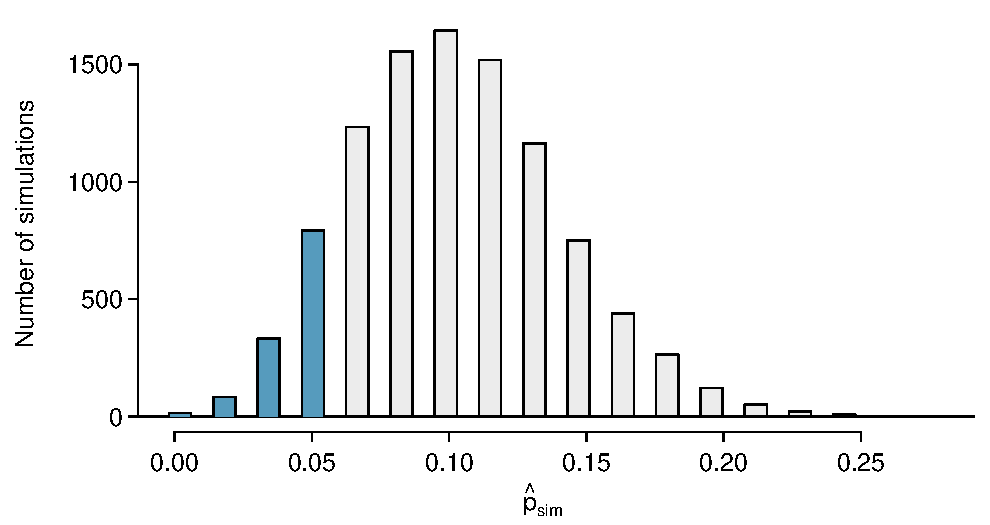
\includegraphics[width=0.9\textwidth]{ch_inference_for_props_oi_biostat/figures/nullDistForPHatIfLiverTransplantConsultantIsNotHelpful/nullDistForPHatIfLiverTransplantConsultantIsNotHelpful}
\caption{The null distribution for $\hat{p}$, created from 10,000 simulated studies. The left tail, representing the p-value for the hypothesis test, contains 12.22\% of the simulations.}
\label{nullDistForPHatIfLiverTransplantConsultantIsNotHelpful}
\end{figure}

\begin{exercise} \label{plainLanguageExplanationOfHTConclusionForLiverDonorSurgicalConsultant}
Because the estimated p-value is 0.1222, which is larger than the significance level 0.05, we do not reject the null hypothesis. Explain what this means in plain language in the context of the problem.\footnote{There isn't sufficiently strong evidence to support an association between the consultant's work and fewer surgery complications.}
\index{data!medical consultant|)}
\end{exercise}

\begin{exercise}
Does the conclusion in Guided Practice~\ref{plainLanguageExplanationOfHTConclusionForLiverDonorSurgicalConsultant} imply there is no real association between the surgical consultant's work and the risk of complications? Explain.\footnote{No. It might be that the consultant's work is associated with a reduction but that there isn't enough data to convincingly show this connection.}
\end{exercise}

\begin{termBox}{\tBoxTitle{One-sided hypothesis test for $p$ with a small sample}
The p-value is always derived by analyzing the null distribution of the test statistic. The normal model poorly approximates the null distribution for $\hat{p}$ when the success-failure condition is not satisfied. As a substitute, we can generate the null distribution using simulated sample proportions ($\hat{p}_{sim}$) and use this distribution to compute the tail area, i.e. the p-value.}
\end{termBox}

We continue to use the same rule as before when computing the p-value for a two-sided test: double the single tail area, which remains a reasonable approach even when the sampling distribution is asymmetric. However, this can result in p-values larger than 1 when the point estimate is very near the mean in the null distribution; in such cases, we write that the p-value is 1. Also, very large p-values computed in this way (e.g. 0.85), may also be slightly inflated.

Guided Practice~\ref{plainLanguageExplanationOfHTConclusionForLiverDonorSurgicalConsultant} said the p-value is \emph{estimated}. It is not exact because the simulated null distribution itself is not exact, only a close approximation. However, we can generate an exact null distribution and p-value using the binomial model from Section~\ref{binomialModel}.

\subsection{Generating the exact null distribution and p-value}
\label{exactNullDistributionUsingBinomialModel}

The number of successes in $n$ independent cases can be described using the binomial model, which was introduced in Section~\ref{binomialModel}. Recall that the probability of observing exactly $k$ successes is given by
\begin{align} \label{binomialEquationShownForFindingNullDistributionInSmallSamplePropTest}
P(k\text{ successes}) = {n\choose k} p^{k}(1-p)^{n-k} = \frac{n!}{k!(n-k)!} p^{k}(1-p)^{n-k}
\end{align}
where $p$ is the true probability of success. The expression ${n\choose k}$ is read as \emph{$n$ choose $k$}, and the exclamation points represent factorials. For instance, $3!$ is equal to $3\times 2\times 1=6$, $4!$ is equal to $4\times 3\times 2\times 1 = 24$, and so on (see Section~\ref{binomialModel}).

The tail area of the null distribution is computed by adding up the probability in Equation~\eqref{binomialEquationShownForFindingNullDistributionInSmallSamplePropTest} for each $k$ that provides at least as strong of evidence favoring the alternative hypothesis as the data. If the hypothesis test is one-sided, then the p-value is represented by a single tail area. If the test is two-sided, compute the single tail area and double it to get the p-value, just as we have done in the past.

\begin{example}{Compute the exact p-value to check the consultant's claim that her clients' complication rate is below 10\%.}
Exactly $k=3$ complications were observed in the $n=62$ cases cited by the consultant. Since we are testing against the 10\% national average, our null hypothesis is $p=0.10$. We can compute the p-value by adding up the cases where there are 3 or fewer complications:
\begin{align*}
\text{p-value}
	&= \sum_{j=0}^{3} {n\choose j} p^{j}(1-p)^{n-j} \\
	&= \sum_{j=0}^{3} {62\choose j} 0.1^{j}(1-0.1)^{62-j} \\
	&= {62\choose 0} 0.1^{0}(1-0.1)^{62-0} +
		{62\choose 1} 0.1^{1}(1-0.1)^{62-1} \\
	& \qquad + {62\choose 2} 0.1^{2}(1-0.1)^{62-2} +
		{62\choose 3} 0.1^{3}(1-0.1)^{62-3} \\
	&= 0.0015 + 0.0100 + 0.0340 + 0.0755 \\
	&= 0.1210
\end{align*}
This exact p-value is very close to the p-value based on the simulations (0.1222), and we come to the same conclusion. We do not reject the null hypothesis, and there is not statistically significant evidence to support the association.

If it were plotted, the exact null distribution would look almost identical to the simulated null distribution shown in Figure~\ref{nullDistForPHatIfLiverTransplantConsultantIsNotHelpful} on page~\pageref{nullDistForPHatIfLiverTransplantConsultantIsNotHelpful}.
\end{example}

\subsection{Using simulation for goodness of fit tests}

Simulation methods may also be used to test goodness of fit. In short, we simulate a new sample based on the purported bin probabilities, then compute a chi-square test statistic $X_{sim}^2$. We do this many times (e.g. 10,000 times), and then examine the distribution of these simulated chi-square test statistics. This distribution will be a very precise null distribution for the test statistic $\chi^2$ if the probabilities are accurate, and we can find the upper tail of this null distribution, using a cutoff of the observed test statistic, to calculate the p-value.

\begin{example}{\index{data!racial make-up of jury|(}Section~\ref{oneWayChiSquare} introduced an example where we considered whether jurors were racially representative of the population. Would our findings differ if we used a simulation technique?}
Since the minimum bin count condition was satisfied, the chi-square distribution is an excellent approximation of the null distribution, meaning the results should be very similar. Figure~\ref{jurorChiSquareSimulated} shows the simulated null distribution using 100,000 simulated $X_{sim}^2$ values with an overlaid curve of the chi-square distribution. The distributions are almost identical, and the p-values are essentially indistinguishable: 0.115 for the simulated null distribution and 0.117 for the theoretical null distribution.
\index{data!racial make-up of jury|)}
\end{example}

\begin{figure}[h]
\centering
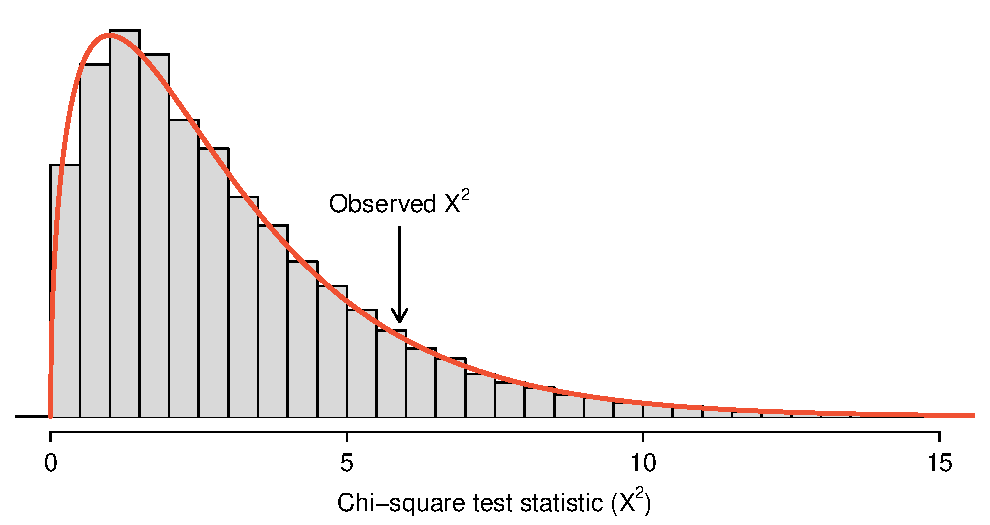
\includegraphics[width=0.9\textwidth]{ch_inference_for_props_oi_biostat/figures/jurorChiSquareSimulated/jurorChiSquareSimulated}
\caption{The precise null distribution for the juror example from Section~\ref{oneWayChiSquare} is shown as a histogram of simulated $X_{sim}^2$ statistics, and the theoretical chi-square distribution is also shown.}
\label{jurorChiSquareSimulated}
\end{figure}

\end{comment}

%__________________
\section{Randomization test (special topic)}
\label{smallSampleHTForTwoOrMoreProportion}

\index{data!CPR and blood thinner|(}

This section discusses the randomization test, a method for conducting inference in a small-sample setting that is based on simulation. The companion to this text covers the details of how to conduct randomization tests in \textsf{R}.

Cardiopulmonary resuscitation (CPR) is a procedure commonly used on individuals suffering a heart attack when other emergency resources are not available. This procedure is helpful for maintaining some blood circulation, but the chest compressions involved can cause internal injuries. Internal bleeding and other injuries complicate additional treatment efforts following arrival at a hospital. For example, blood thinners are commonly administered to release a clot responsible for triggering a heart attack. However, blood thinners would exacerbate any internal bleeding. The results of the study are shown in Table~\ref{resultsForCPRStudyInSmallSampleSection}.

\begin{table}[ht]
	\centering
	\begin{tabular}{lccccc}
		\hline
		&& Survived 	& Died 	&& Total \\
		\hline
		Control		&& 11		& 39		&& 50 \\
		Treatment		&& 14		& 26		&& 40 \\
		\hline
		Total			&& 25		& 65		&& 90 \\
		\hline
	\end{tabular}
	\caption{Results for the CPR study. Patients in the treatment group were given a blood thinner, and patients in the control group were not.}
	\label{resultsForCPRStudyInSmallSampleSection}
\end{table}

\begin{exercise} What is an appropriate set of hypotheses for this study? \footnote{The null hypothesis is that the survival rate in the control group ($p_c$) is equal to the survival rate in the treatment group ($p_t$), i.e. $H_0: p_c = p_t$. The null is tested against the alternative, that blood thinners have an overall survival effect, $H_A: p_c \neq p_t$. Alternatively, the hypothesis can be stated in terms of a $\chi^2$ framework. The null hypothesis that treatment is independent of outcome is tested against an alternative that treatment and outcome are associated.}
\end{exercise}

\subsection{Large sample framework for a difference in two proportions}

When sample sizes are large, it is reasonable to use an inference approach that relies on approximation. The point estimate of the difference in survival proportions of the two groups, $\hat{p}_t - \hat{p}_c$, can be adequately modeled using a normal approximation. The expected umber of successes (13.9, 11.1) and failures (36.1, 28.9) are above 10, which satisfies the success-failure condition. Additionally, it can be assumed that patients are independent.

\begin{example}{Assess the significance of the data in Table~\ref{resultsForCPRStudyInSmallSampleSection} against a two-sided alternative. Use $\alpha = 0.05$. }

Calculate the pooled proportion, $\hat{p}$: 
\[\hat{p} = \dfrac{11 + 14}{50 + 40} = 0.278\]
	
Calculate the test statistic, $z$:

\[z = \dfrac{0.35 - 0.22 }{0.278(1-0.278)\sqrt{\frac{1}{40} + \frac{1}{50}}} =  1.37\]
	
This $z$-score has area 0.0853 in the right tail. The $p$-value is 0.176, twice the single-tail area. There is insufficient evidence to reject the null hypothesis that there is a difference in survival rates between the treatment and control groups.\footnote{It is also valid to use a $\chi^2$ test to assess significance. The $\chi^2$ statistic of 1.87 and degrees of freedom 1 corresponds to a $p$-value between 0.1 and 0.2. From software, the exact $p$-value is 0.17.}

%chi-squarate p-value without continuity correction	

\begin{figure}[ht]
	\centering
	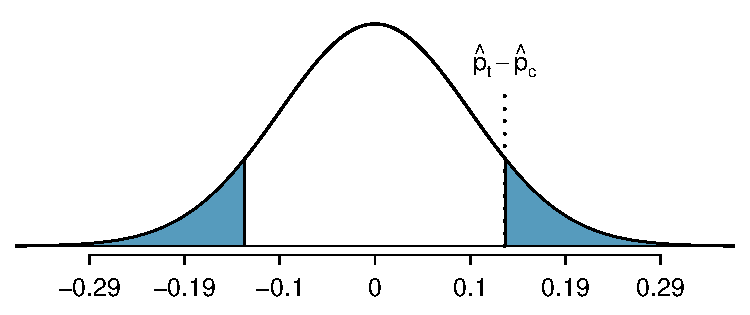
\includegraphics[width=0.67\textwidth]{ch_inference_for_props_oi_biostat/figures/pValueCPRStudyLargeSampleAnalysisInSmallSampleSection/pValueCPRStudyLargeSampleAnalysisInSmallSampleSection}
	\caption{The null distribution of the point estimate $\hat{p}_t - \hat{p}_c$ under the large sample framework is a normal distribution with mean $0$ and standard deviation equal to the standard error.}
	\label{pValueCPRStudyLargeSampleAnalysisInSmallSampleSection}
\end{figure}

\end{example}


The $p$-value 0.176 relies on the normal approximation. When sample sizes are relatively small, and expected values are fairly close to 10, the approximation may only be adequate. The following section describes a simulation technique that produces more accurate $p$-values.

\subsection{Small sample framework for a difference in two proportions}

Under the null hypothesis, a patient is equally likely to survive whether they are in the control group or the treatment group. A simulation can be run to produce a set of results that might occur if the null hypothesis is true, where the expected difference between $p_c$ and $p_t$ is zero.

Assume that the numbers of patients who survived and died remain constant. However, randomly assign 40 \resp{control\_sim} and \resp{treatment\_sim} labels to the patients; these label counts correspond to the number of patients assigned to each group in the actual study. The simulation results of one such simulation are shown in Table~\ref{resultsForCPRStudyInSmallSampleSectionFake1}.

\begin{table}[ht]
\centering
\begin{tabular}{lccccc}
\hline
			&& Survived 	& Died 	&& Total \\
\hline
\resp{control\_sim}		&& 15		& 35		&& 50 \\
\resp{treatment\_sim}	&& 10		& 30		&& 40 \\
\hline
Total			&& 25		& 65		&& 90 \\
\hline
\end{tabular}
\caption{Simulated results for the CPR study under the null hypothesis. The labels were randomly assigned and are independent of the outcome of the patient.}
\label{resultsForCPRStudyInSmallSampleSectionFake1}
\end{table}

\begin{exercise} \label{exerciseComputingDifferenceForCPRStudyInSmallSampleSectionFake1}
What is the difference in survival rates between the two groups in Table~\ref{resultsForCPRStudyInSmallSampleSectionFake1}? How does this compare to the observed 13\% in the real groups?\footnote{The difference is $\hat{p}_{t, sim} - \hat{p}_{c, sim} = \frac{10}{40} - \frac{15}{50} = -0.05$, which is closer to the null value $p_0=0$ than what was observed.}
\end{exercise}

The difference computed in Guided Practice~\ref{exerciseComputingDifferenceForCPRStudyInSmallSampleSectionFake1} represents a draw from the null distribution of the sample differences. To build the complete null distribution of the sample differences, it is necessary to generate many more simulated experiments.

The null distribution constructed from 10,000 simulations is shown in Figure~\ref{pValueCPRStudySmallSampleAnalysisInSmallSampleSection}. The shaded tail region representing draws with differences $\hat{p}_t - \hat{p}_c$ more extreme than 0.13 has area 0.13; the $p$-value equals 0.26. The normal approximation produced a $p$-value of 0.176, which is relatively far from the value obtained with the randomization approach, although the conclusions of the test are the same in both cases. 

\begin{figure}[ht]
\centering
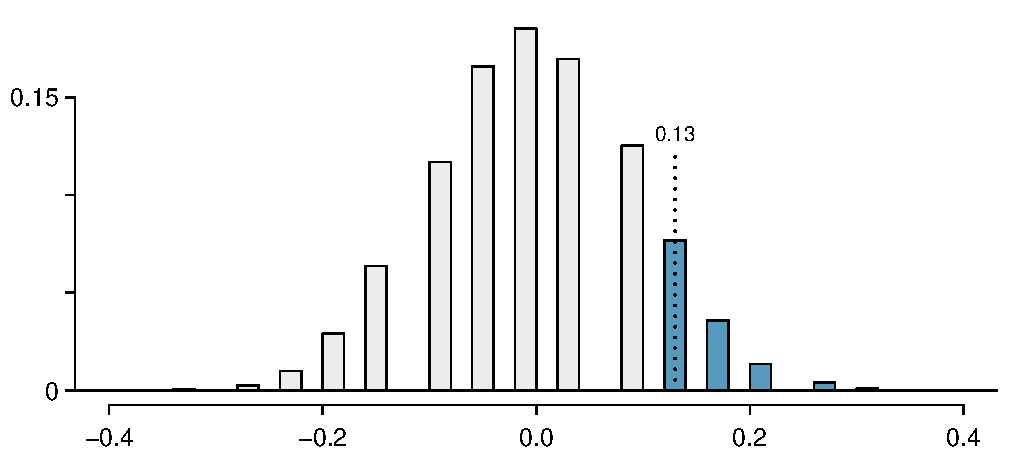
\includegraphics[width=\textwidth]{ch_inference_for_props_oi_biostat/figures/pValueCPRStudySmallSampleAnalysisInSmallSampleSection/pValueCPRStudySmallSampleAnalysisInSmallSampleSection}
\caption{An approximation of the null distribution of the point estimate, $\hat{p}_t - \hat{p}_c$. The p-value is twice the right tail area.}
\label{pValueCPRStudySmallSampleAnalysisInSmallSampleSection}
\end{figure}

In general, small sample methods produce more accurate results since they rely on fewer assumptions. However, they often require doing additional computation or resorting to simulation methods. For this reason, small sample methods are typically used only when conditions for large sample methods are not satisfied.

\subsection{Randomization for two-way tables}

Randomization methods may also be used for contingency tables. This involves creating randomized contingency tables and computing $\chi^2$ statistics, then examining the null distribution. This randomization approach is valid for any sized sample, and it will be more accurate for cases where one or more expected bin counts do not meet the minimum threshold of~5. When the minimum threshold is met, the simulated null distribution will very closely resemble the $\chi^2$ distribution. 